%% ---------------------------------------------------------------------------
%%  Neurocomputing (Elsevier) submission version of SCORE-Net
%%  Class: elsarticle (Elsevier). Reference style: Elsevier numbered.
%%
%%  Build:   latexmk -pdf main.tex      (or ./build.sh)
%%  NOTE:    All files of the flattened submission archive must sit in ONE
%%           folder; Editorial Manager cannot process subfolders.
%% ---------------------------------------------------------------------------
\documentclass[5p,10pt]{elsarticle}

% --- Encoding and fonts ---
\usepackage[utf8]{inputenc}
\usepackage[T1]{fontenc}

% --- Mathematics ---
\usepackage{amsmath,amsthm}
\usepackage{amssymb}

% --- Times-like fonts (matches Elsevier's published style) ---
\usepackage{newtxtext}
\usepackage{newtxmath}

% --- Graphics and tables ---
\usepackage{graphicx}
\usepackage{booktabs}
\usepackage{tabularx}
\usepackage{multirow}
\usepackage{adjustbox}

% --- Misc ---
\usepackage{url}
\usepackage{microtype}
\usepackage{algorithm}
\usepackage{algpseudocode}
\usepackage[hidelinks]{hyperref}
% Allow long DOIs/URLs in the reference list to break at any character.
\usepackage{xurl}

% Narrow two-column measure: let TeX stretch interword space a little before
% it produces an overfull line.
\setlength{\emergencystretch}{2em}

% --- Float placement tuning ---
% Double-column floats (table*, figure*) need two things that the elsarticle
% defaults do not provide:
%   * dblfloatfix: respects [b] for double-column floats. Without it, a float
%     declared [!b] is silently ignored and is deferred to the end of the
%     document, i.e. after the reference list.
%   * a raised \dbltopnumber: by default only two double-column floats may sit
%     at the top of a page, so a paper with 17 of them backs up and the queue
%     is flushed by \end{document}, again after the references.
\usepackage{dblfloatfix}
\setcounter{dbltopnumber}{3}
\renewcommand{\dbltopfraction}{0.9}
\renewcommand{\dblfloatpagefraction}{0.75}
\renewcommand{\topfraction}{0.95}
\renewcommand{\bottomfraction}{0.95}
\renewcommand{\textfraction}{0.05}
\renewcommand{\floatpagefraction}{0.85}

% --- Theorem environments ---
\newtheorem{theorem}{Theorem}
\newtheorem{lemma}[theorem]{Lemma}
\newtheorem{proposition}[theorem]{Proposition}
\newtheorem{definition}{Definition}
\newtheorem{remark}{Remark}

% --- Custom macros ---
\newcommand{\modelname}{\textsc{SCORE-Net}}
\newcommand{\R}{\mathbb{R}}
\newcommand{\E}{\mathbb{E}}

\journal{Neurocomputing}

% Many floats: allow pages to end short instead of stretching the body
% to the exact bottom, which produced an overfull vbox on float-heavy pages.
\raggedbottom

\begin{document}

\begin{frontmatter}

\title{\modelname: Inherently Interpretable Tabular Classification via
Localized Convex Slabs}

%% Author affiliation verified against the Sakarya University staff directory
%% (seng.sakarya.edu.tr) and the authors' public ORCID records.
\author[a]{Ahmet Alkan\corref{cor1}\fnref{orcidA}}
\ead{ahmetalkan@sakarya.edu.tr}
\fntext[orcidA]{ORCID: 0009-0006-4919-8080.}
\author[a]{Gozde Yolcu Oztel\fnref{orcidB}}
\ead{gyolcu@sakarya.edu.tr}
\fntext[orcidB]{ORCID: 0000-0002-7841-2131.}
\cortext[cor1]{Corresponding author.}
\address[a]{Department of Software Engineering, Faculty of Computer and
Information Sciences, Sakarya University, Esentepe Campus, 54187 Serdivan,
Sakarya, Turkey}

\begin{abstract}
Machine learning is increasingly used for high-stakes decisions, where
transparency is required. Tree ensembles and deep networks are accurate on tabular
data but hard to inspect, and post-hoc tools such as SHAP and LIME are only
local. Simpler transparent models struggle with non-linear interactions without
growing too large to audit. We propose \modelname{} (Self-explaining Convex Operational Rule Engine), an
inherently interpretable neural network for tabular classification. It replaces
unbounded activations with localized triangular activations on bias-free linear
projections, so every hidden unit defines a convex slab between two parallel
hyperplanes: an interval rule with compact support and a signed vote per class.
Dual $\ell_1$ regularization and iterative magnitude pruning keep the rule set
small. We prove an \emph{exact bias-shifting property}: a rule pruned to zero
weights has a constant baseline activation that can be absorbed into the output
bias without changing predictions. Rule-adaptive integer quantization turns
projection weights into small integers while the output layer stays continuous,
so small rule sets can be scored by hand. We evaluate on COMPAS, German Credit, UCI Adult and a 20-class synthetic task.
On the three binary datasets, compact models keep 5--46 rules with 1.2--2.7
features per rule and 96.0--98.7\% sparsity, and the single split stays within
2.5 points of the best of 13 baselines; under cross-validation COMPAS trails
CatBoost by 0.4--1.1 points and German Credit by 2.8--3.1. On the synthetic task
the models lead all baselines. Integer scorecards retain 95.45--100\% prediction
agreement.

\end{abstract}

\begin{keyword}
Interpretable machine learning \sep Explainable artificial intelligence \sep
Tabular data \sep Scorecards \sep Neural network pruning \sep
Trustworthy artificial intelligence
\end{keyword}

\end{frontmatter}

% --- Section 1: Introduction ---
\section{Introduction}
\label{sec:introduction}

Tabular data is one of the most common data formats in practical applications \cite{Lee2024,Mahendra2026}. It is widely used in high-stakes fields such as credit scoring, loan approvals, criminal recidivism risk assessment, and clinical decision support~\cite{rudin2019stop,caruana2015intelligible,zeng2017interpretable}. In these domains, model predictions directly affect people's lives and financial well-being. Over the past decade, ensemble methods---such as XGBoost~\cite{chen2016xgboost}, LightGBM~\cite{ke2017lightgbm}, and CatBoost~\cite{prokhorenkova2018catboost}---as well as deep neural networks and, most recently, tabular foundation models~\cite{hollmann2025tabpfn} have achieved strong predictive performance on tabular benchmarks. However, these models offer limited transparency into how they reach a prediction. Many act as ``black boxes'' with complex internal structures, so domain experts cannot easily inspect how a specific decision is made.

The need for model transparency is reinforced by legal regulations such as the European Union Artificial Intelligence Act (EU AI Act)~\cite{eu2024ai} and the General Data Protection Regulation (GDPR)~\cite{wachter2017counterfactual}. These laws increasingly require automated decision systems to provide meaningful explanations to affected individuals. To meet this requirement, researchers commonly turn to post-hoc explanation methods such as SHAP~\cite{lundberg2017unified} and LIME~\cite{ribeiro2016why}. However, these explanations do not necessarily reveal how the model actually decides, and they can suffer from limited faithfulness, high computational cost, or vulnerability to adversarial manipulation~\cite{rudin2019stop,slack2020fooling}.

Consequently, interest has grown in \emph{inherently interpretable} (or ``glass-box'') models, in which transparency is built into the architecture itself. Yet glass-box models face a hard trade-off between predictive power and simplicity. Linear models cannot capture complex feature interactions, while deep decision trees quickly grow too large to follow. Generalized additive models become computationally heavy in multi-class settings, and discrete integer scorecards are hard to optimize at scale. Domain experts are thus caught between the high accuracy of neural networks and the practical clarity of rule-based scorecards.


To bridge this divide, we propose \modelname{} (\textbf{S}elf-explaining \textbf{C}onvex \textbf{O}perational \textbf{R}ule \textbf{E}ngine), an inherently interpretable neural network for tabular classification. \modelname{} combines the gradient-based training of neural networks with the operational simplicity of rule-based scorecards.


The central idea behind \modelname{} is geometric. Instead of letting each hidden
unit respond over an unbounded region of the input space, the architecture
confines every unit to a localized convex slab. Each unit therefore behaves as an
inspectable interval rule with a bounded firing region. A linear output layer
aggregates the firing strengths of these rules into signed class scores. Thus any
single prediction can be written as a baseline term plus a small number of rule
contributions. To keep the rule set compact, the model is regularized and structurally pruned. The surviving rules can optionally be converted into small integer scorecards. When the rule set is small enough, such a scorecard can be evaluated by hand, while larger rule sets remain inspectable rule by rule.

The contribution is therefore best read as an \emph{explainability} result rather
than a new accuracy frontier. Localized activations, magnitude pruning, and integer scorecards all exist in the literature. We examine whether they can be combined into a single model whose decisions remain inspectable end to end. We also investigate the predictive performance trade-offs associated with this combination. Each design
choice follows from this goal. The bias-free projection gives pruning a clean
semantic meaning, the pruning schedule shortens rules rather than merely
compressing the network. The quantization step keeps each rule small enough
to inspect and, for compact models, to score by hand. The experiments report
where the retained transparency costs accuracy and where it does not. They also include a
variant of the recidivism benchmark with the legally protected attributes
removed.

The main contributions of this paper are summarized as follows:

\begin{enumerate}
    \item \textbf{Localized Convex Slab Neural Architecture:} We introduce \modelname{}, an end-to-end differentiable glass-box architecture for tabular classification. By combining bias-free feature projections with localized triangular activations, each hidden neuron represents an inspectable rule defined over a bounded convex slab.
    \item \textbf{Exact Bias Shifting for Pruned Rules:} We state and prove an exact identity, showing that structurally empty rules from magnitude pruning can be absorbed into the output layer bias with zero change in model predictions.
    \item \textbf{Rule-Level Integer Scorecard Formulation:} We develop a rule-adaptive
    quantization procedure that maps continuous projection weights into low-magnitude
    integers, turning each rule into a transparent scorecard entry that retains
    95.45--100\% prediction agreement with the float model.
    \item \textbf{Empirical Evaluation and Tools:} We evaluate \modelname{} on four
    benchmarks against 13 baselines with a validation-only selection protocol. Two
    post-hoc operating points are test-informed and declared explicitly in
    Section~\ref{subsubsec:protocol}. We report bootstrap confidence intervals,
    McNemar tests and repeated stratified cross-validation for every model and
    dataset. We also provide closed-form tools for local decision decomposition, global
    feature influence and geometric recourse. Thus, a fitted model can be inspected
    without a surrogate explainer.
\end{enumerate}


The remainder of this paper is organized as follows.
Section~\ref{sec:related_work} reviews interpretable tabular learning, neural rule
representations, pruning, scorecards, and post-hoc methods.
Section~\ref{sec:methodology} presents the formulation, the convex slab geometry,
the exact bias-shifting property, the quantization algorithm, and the analytical
interpretability tools. Section~\ref{sec:experiments} reports the experimental
setup, benchmarks, pruning behavior, quantization fidelity, and case studies.
Section~\ref{sec:conclusion} concludes and outlines future work.


% --- Section 2: Related Work ---
\section{Related Work}
\label{sec:related_work}

\subsection{Inherently Interpretable Tabular Models}
\label{subsec:related_interpretable}

Inherently interpretable (glass-box) models expose their decision logic without a
separate post-hoc explainer~\cite{rudin2019stop}; reviews of the tabular setting
\cite{obrien2024explainable} and of how such explanations are evaluated
\cite{nauta2023evaluating} give broader context.

\textbf{Linear and generalized linear models.} Linear and logistic regression are
among the oldest interpretable models, and each coefficient reads as the marginal
effect of a feature on the log-odds. They cannot represent non-linearities or
interactions without manual feature engineering.

\textbf{Decision trees and rule sets.} Trees and rule-based systems offer intuitive
\emph{IF--THEN} rules~\cite{wang2017bayesian,friedman2008predictive}, but reaching
competitive accuracy requires deep trees that are hard to follow, and axis-aligned
splits handle diagonal or correlated boundaries poorly.

\textbf{Generalized additive models.} GAMs decompose predictions into univariate
shape functions, $g(E[Y]) = \beta_0 + \sum f_i(x_i)$. Explainable Boosting
Machines~\cite{lou2012intelligible,caruana2015intelligible} add pairwise
interactions by shallow tree boosting, and Neural Additive
Models~\cite{agarwal2021neural} model each shape function with a small network.
Their cost grows sharply with many correlated features, many classes, and
higher-order interactions.

\subsection{Neural Rule Representations and Localized Activations}
\label{subsec:related_neural_rules}

Prototype networks~\cite{chen2019looks} and Radial Basis Function (RBF) networks
activate hidden units through distance-based centroids. Standard RBFs use isotropic
Euclidean distances that decay smoothly, so every neuron stays slightly active
everywhere. Piecewise-linear, compact-support activations instead drop to exactly
zero outside a defined region. Localized triangular (tent) activations suit such
units, but they have rarely been combined with bias-free projections and structural
pruning to extract discrete rule sets for tabular data. Sparse tabular neural
networks pursue a related goal with different mechanisms~\cite{raieli2026escaping}.
\modelname{} uses this geometry so that each neuron isolates a \emph{convex slab},
an explicit interval condition rather than an unbounded response.

\subsection{Neural Network Pruning and Structural Sparsity}
\label{subsec:related_pruning}

Neural network pruning was originally developed to compress large models and reduce memory and latency on hardware accelerators~\cite{han2015learning}. The Lottery Ticket Hypothesis by Frankle and Carbin~\cite{frankle2018lottery} demonstrated that dense, randomly initialized neural networks contain sparse sub-networks (``winning tickets'') that can reach comparable test accuracy when trained in isolation.

In \modelname{}, we use Iterative Magnitude Pruning (IMP) not only to compress the model but as a \emph{semantic sparsification mechanism}. In our architecture, setting an input connection $W_{f,hj}$ to zero directly removes feature $j$ from rule $h$, which shortens the rule. Also, when all input connections to a neuron are zeroed, the whole rule becomes inactive. Unlike conventional pruning pipelines that discard pruned units heuristically, we give a formal statement---the \emph{exact bias shifting for pruned rules}---which guarantees that disconnected rules can be absorbed into the output bias without altering model outputs.

\subsection{Scoring Systems and Integer Scorecards}
\label{subsec:related_scorecards}

Point-based scoring systems (scorecards) have been used for decades in medicine (e.g., the CHADS$_2$ score for stroke risk~\cite{gage2001validation}) and finance (e.g., credit bureau scorecards~\cite{hlongwane2024transparency}). In a scorecard, integer points are assigned to specific conditions, and the user simply adds the points together to obtain a risk category.

Modern methods such as Supersparse Linear Integer Models (SLIM)~\cite{ustun2016supersparse} and RiskSLIM~\cite{ustun2017optimized}, which has been applied to recidivism prediction~\cite{zeng2017interpretable}, train scorecards as a discrete optimization problem using Mixed-Integer Non-Linear Programming (MINLP). These methods produce provably optimal and highly sparse scorecards, but solving MINLP is NP-hard. As a result, training becomes very slow on datasets with many samples, many features, or multi-class targets. \modelname{} avoids this bottleneck by first training the continuous model with standard gradient descent and iterative pruning, and then converting the resulting compact rules into an integer scorecard via rule-adaptive scaling. The resulting prediction agreement is high but empirical rather than exact, and it is measured on the test partition. The recourse tool is likewise geometric rather than causal, a distinction that the counterfactual literature emphasizes~\cite{verma2024counterfactual}.

\subsection{Post-Hoc Explanations vs. Inherently Interpretable Models}
\label{subsec:related_posthoc}

Post-hoc explainability methods, particularly SHAP~\cite{lundberg2017unified} and LIME~\cite{ribeiro2016why}, have become a common way to explain black-box models. These tools build local surrogate models around individual predictions to estimate feature attributions.

Despite their popularity, post-hoc methods have fundamental limitations in
high-stakes domains~\cite{rudin2019stop}. They explain an approximation of the
model rather than its decision logic, so a diverging surrogate can mislead.
Estimating Shapley values is computationally expensive, and sampling-based
perturbations generate out-of-distribution points that distort attributions; the
same concern motivates dedicated evaluation protocols~\cite{nauta2023evaluating}.
Finally, some explainers can be fooled by adversarial wrappers that change the
explanation without changing the prediction~\cite{slack2020fooling}.

These limitations motivate inherently interpretable models such as \modelname{},
whose explanations are derived analytically from the model parameters.

\subsection{Positioning \modelname{} in the Literature}
\label{subsec:related_positioning}

Localized activations, magnitude pruning and integer scorecards all exist in
isolation. \modelname{} combines them so that the combination, rather than any
single component, carries the interpretability claim: bias-free projections with
triangular activations yield bounded convex-slab rules; pruning is semantic rather
than merely compressive and is backed by exact bias shifting; post-training
quantization produces integer scorecards without discrete optimization; and
decision decomposition, feature influence and recourse are available in closed
form. Relative to linear scorecards and GAMs, the representation is piecewise
linear and oblique, which is what allows it to cover localized non-axis-aligned
regions; relative to tree ensembles and deep networks, it exposes each decision as
a small number of signed rule votes rather than a surrogate explanation.


% --- Section 3: Methodology ---
\section{Methodology}
\label{sec:methodology}


\subsection{Architectural Formulation of \modelname{}}
\label{subsec:architecture}

Let $\mathcal{D} = \{(x_i, y_i)\}_{i=1}^M$ denote a tabular dataset with $M$ samples, where each input vector $x_i = [x_{i1}, x_{i2}, \dots, x_{iN}]^\top \in \R^N$ contains $N$ features, and $y_i \in \{1, 2, \dots, C\}$ represents the target class label across $C$ discrete categories. 

\modelname{} is a three-layer feedforward architecture with interpretable internal states,
shown in Figures~\ref{fig:arch_forward}--\ref{fig:arch_scorecard} together with the
activation function and the scorecard entries it produces:
\begin{enumerate}
    \item A bias-free linear feature projection layer,
    \item A localized triangular activation layer with learnable centers and widths,
    \item A linear output scoring layer producing class logits.
\end{enumerate}

\begin{figure*}[t]
\centering
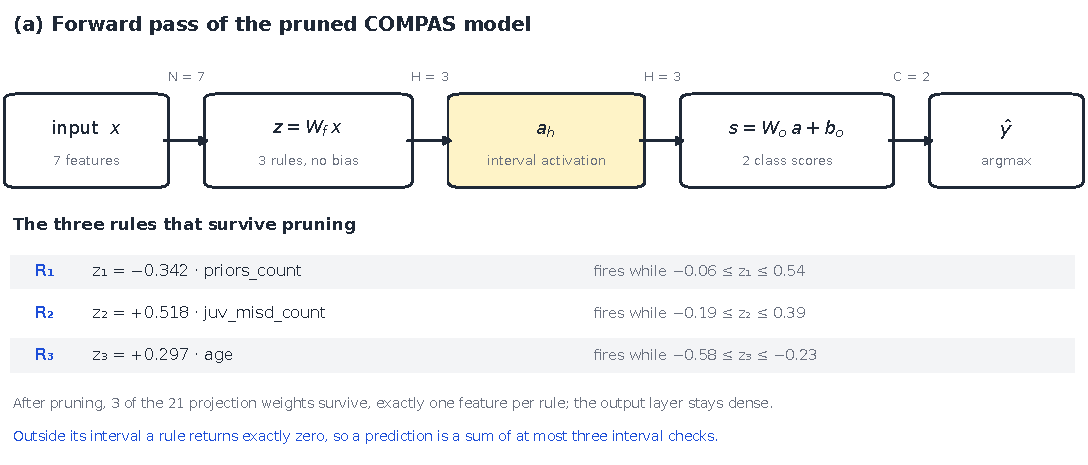
\includegraphics[width=\textwidth]{figures/fig_arch_forward.pdf}
\caption{The \modelname{} forward pass for the protected-attribute-free COMPAS
variant of Section~\ref{subsec:comparative_results}, drawn from its released Compact
checkpoint. A bias-free projection $W_f \in \R^{3 \times 7}$ maps the $N=7$ inputs to
$H=3$ scalars $z_h$; each scalar is passed through a localized activation $a_h$; a
linear output layer maps the three activations to $C=2$ class scores, and the larger
score gives the prediction. The table lists the three rules that survive pruning,
with the weight and firing interval read from the checkpoint.}
\label{fig:arch_forward}
\end{figure*}

\begin{figure*}[t]
\centering
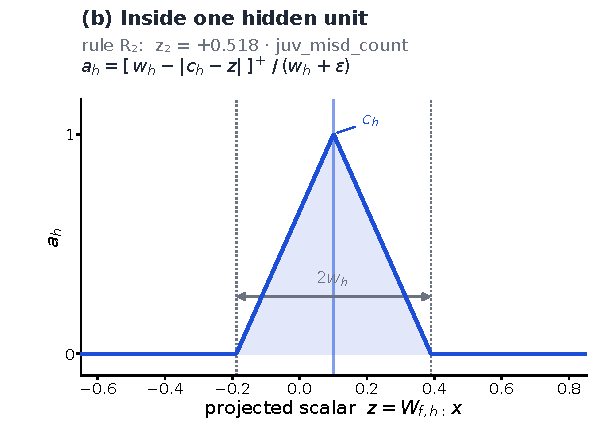
\includegraphics[width=0.55\textwidth]{figures/fig_arch_unit.pdf}
\caption{The activation of a single hidden unit as a function of the projected scalar
$z=W_{f,h:}x$. It peaks at $c_h$, decreases linearly, and is exactly zero for
$|c_h - z| \ge w_h$, so the unit is active only on an interval of width $2w_h$. The
plotted parameters belong to rule $R_2$ of the same Compact model
(the protected-attribute-free COMPAS variant).}
\label{fig:arch_unit}
\end{figure*}

\begin{figure*}[t]
\centering
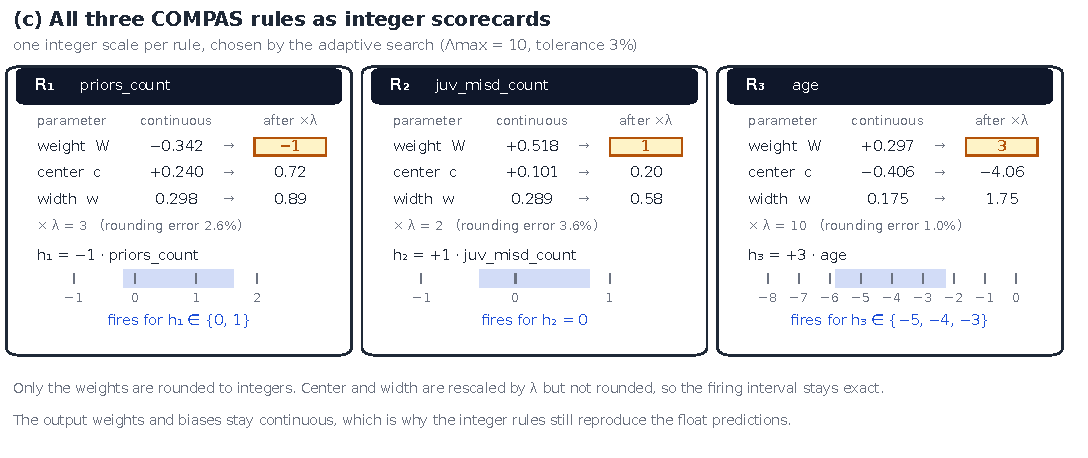
\includegraphics[width=\textwidth]{figures/fig_arch_scorecard.pdf}
\caption{Rule-level integer quantization applied to all three rules of the same
COMPAS Compact model. Each rule
uses its own scale $\lambda_h$, chosen by the adaptive search of
Section~\ref{subsec:scorecard} (the budget is printed in the panel): the continuous
weight $W$ is multiplied by $\lambda_h$ and rounded to the small integer in the shaded
box, while the center $c$ and width $w$ are rescaled by the same $\lambda_h$ but not
rounded, so the firing interval stays exact. Each card shows the integer point sum
$h_h$ and the integer values it must take for the rule to fire. The output layer $W_o$
and the bias $b_o$ remain continuous.}
\label{fig:arch_scorecard}
\end{figure*}

\subsubsection{Layer 1: Bias-Free Linear Projection}
Given an input sample $x \in \R^N$, the model first computes $H$ linear combinations using a weight matrix $W_f \in \R^{H \times N}$:
\begin{equation}
\label{eq:linear_projection}
h = W_f x, \quad \text{where } h_h = \sum_{j=1}^N W_{f,hj} x_j, \quad \forall h \in \{1, \dots, H\}.
\end{equation}
In this equation, each row $W_{f,h:} \in \R^N$ acts as a feature projection vector for the $h$-th hidden neuron. 

We omit a bias term in this layer ($bias = \text{False}$). As a result, when the input is zero ($x = 0$), the projection is also zero ($h = 0$). As we show in Section~\ref{subsec:bias_shifting}, this choice matters: when a rule's input connections are pruned to zero, its baseline behavior becomes a constant that does not depend on the input, and it can be absorbed exactly into the output bias.


\subsubsection{Layer 2: Localized Triangular Rule Activation}
Standard neural networks typically use monotonic activations such as ReLU ($\max(0, z)$), which stay active over unbounded regions of the input space. In contrast, \modelname{} equips each hidden unit $h$ with two learnable scalar parameters: a center $c_h \in \R$ and an unconstrained base width parameter $\tilde{w}_h \in \R$. We define the operational half-width $w_h$ as the magnitude of the base width,
\begin{equation}
w_h = |\tilde{w}_h|,
\end{equation}
so that the effective bandwidth is strictly positive whenever $\tilde{w}_h \neq 0$.

The localized triangular activation $\text{Act}_h(x)$ is defined as:
\begin{equation}
\label{eq:triangular_activation}
a_h(x) = \text{Act}_h(x) = \frac{\max\Big(0, \, w_h - |c_h - h_h|\Big)}{w_h + \epsilon},
\end{equation}
where $\epsilon = 10^{-8}$ is a small constant added to the denominator to avoid division by zero when the base width collapses to zero; it does not change the support of the rule.

The activation has three useful properties (Figure~\ref{fig:arch_unit}):
\begin{itemize}
    \item \textbf{Bounded Output Range:} $a_h(x) \in [0, 1]$ for all $x \in \R^N$.
    \item \textbf{Centroid Peak:} When the projection exactly matches the center ($h_h = c_h$), the activation reaches its maximum value $a_h(x) = w_h/(w_h+\epsilon)$, which equals $1$ up to the $10^{-8}$ denominator regularizer.
    \item \textbf{Compact Support (Hard Zero Region):} When the distance between the projection and the center is at least the width ($|c_h - h_h| \ge w_h$), the activation is identically zero ($a_h(x) = 0.0$).
\end{itemize}

During training, an optional dropout mask with probability $p_{drop}$ is applied to the activation vector $a(x) = [a_1(x), \dots, a_H(x)]^\top$ to prevent co-adaptation among redundant rules.

\subsubsection{Layer 3: Class-Specific Logit Scoring}
The activation vector $a(x) \in \R^H$ is fed into a linear classification layer parameterized by a weight matrix $W_o \in \R^{C \times H}$ and a class bias vector $b_o \in \R^C$. The unnormalized class score (logit) for class $c \in \{1, \dots, C\}$ is computed as:
\begin{equation}
\label{eq:output_scoring}
s_c(x) = b_{o,c} + \sum_{h=1}^H W_{o,ch} \, a_h(x).
\end{equation}

The output layer is trained without a bias parameter, so the logits depend only on the
rule activations. As shown in Section~\ref{subsec:bias_shifting}, the bias vector $b_o$
is created during post-training compaction, when the constant baseline activations of
pruned rules are absorbed into it.

The coefficient $W_{o,ch}$ is the signed vote that rule $h$ casts for class $c$. A positive value adds evidence for class $c$ when the rule fires; a negative value counts against class $c$.

The final predicted class label $\hat{y}$ is obtained via the argmax operator:
\begin{equation}
\hat{y} = \arg\max_{c \in \{1, \dots, C\}} s_c(x).
\end{equation}

The softmax transformation converts the class logits into normalized class probability estimates:
\begin{equation}
P(Y = c \mid x) = \frac{\exp(s_c(x))}{\sum_{k=1}^C \exp(s_k(x))}.
\end{equation}


\subsection{Geometric Characterization: Localized Convex Slabs}
\label{subsec:geometry}

To understand what a hidden unit represents, we characterize the region in the input space $\R^N$ on which it is active.

\begin{definition}[Localized Convex Slab Rule]
For any hidden unit $h \in \{1, \dots, H\}$ with projection vector $W_{f,h:} \in \R^N$, center $c_h$, and width $w_h > 0$, the activation is strictly positive on the open slab $c_h - w_h < \sum_j W_{f,hj} x_j < c_h + w_h$ and exactly zero elsewhere. Its \emph{closed support}---the closure of that set, i.e.\ the inputs on which the rule fires or reaches its boundary---is the convex slab
\begin{equation}
\label{eq:convex_slab}
\mathcal{S}_h = \left\{ x \in \R^N : c_h - w_h \le \sum_{j=1}^N W_{f,hj} x_j \le c_h + w_h \right\}.
\end{equation}
\end{definition}


In classical rule systems such as decision tree leaves, a rule is an axis-aligned
hyperrectangle $\bigwedge_j (l_j \le x_j \le u_j)$. Unless $W_{f,h:}$ has a single
non-zero entry, $\mathcal{S}_h$ is instead a \textbf{convex slab}: the closed
region between two parallel hyperplanes orthogonal to $W_{f,h:}$. When pruning
leaves one active feature, the slab becomes a 1D interval, $x_j$ lying between
$(c_h-w_h)/W_{f,hj}$ and $(c_h+w_h)/W_{f,hj}$ (swapped when $W_{f,hj}<0$); with
two features it is an oblique strip. \modelname{} therefore generalizes
axis-aligned interval rules to oblique ones while retaining sharp geometric
boundaries.


\subsubsection{Piecewise Linearity and Breakpoints}
Along the one-dimensional projected coordinate $z = W_{f,h:} x$, the activation function $a_h(z)$ is continuous and piecewise linear, with exactly three derivative breakpoints:
\begin{equation}
z \in \{ c_h - w_h, \; c_h, \; c_h + w_h \}.
\end{equation}
The derivative of the activation with respect to the projected input $z$ is:
\begin{equation}
\frac{\partial a_h}{\partial z} = 
\begin{cases}
+1 / (w_h + \epsilon), & \text{if } c_h - w_h < z < c_h, \\
-1 / (w_h + \epsilon), & \text{if } c_h < z < c_h + w_h, \\
0, & \text{if } z < c_h - w_h \text{ or } z > c_h + w_h.
\end{cases}
\end{equation}
This piecewise-linear structure ensures that the entire network maps the input space into hyperplane-bounded response regions, which makes exact sensitivity analysis and boundary verification straightforward.


\subsection{Training Protocol and Structural Sparsification}
\label{subsec:pruning}

To obtain a compact and human-auditable rule set, we train \modelname{} through a two-stage process: regularized optimization followed by Iterative Magnitude Pruning (IMP).

\subsubsection{Regularized Loss Function}
We train the network end-to-end using standard gradient descent. The total training objective combines the cross-entropy classification loss with dual $\ell_1$ regularization penalties~\cite{tibshirani1996lasso} on both weight layers:
\begin{equation}
\label{eq:total_loss}
\mathcal{L}(\theta) = \mathcal{L}_{CE}(y, s(x)) + \lambda_1 \|W_f\|_1 + \lambda_2 \|W_o\|_1,
\end{equation}
where $\mathcal{L}_{CE}$ is the standard multiclass cross-entropy:
\begin{equation}
\mathcal{L}_{CE} = - \frac{1}{M} \sum_{i=1}^M \sum_{c=1}^C \mathbb{I}(y_i = c) \log \left( \frac{\exp(s_c(x_i))}{\sum_{k=1}^C \exp(s_k(x_i))} \right).
\end{equation}
The $\ell_1$ penalty on $W_f$ encourages sparsity in feature connections, driving redundant feature weights to zero and reducing the number of variables in each rule. The $\ell_1$ penalty on $W_o$ encourages the network to use only a minimal subset of rules for class scoring.

\subsubsection{Iterative Magnitude Pruning (IMP)}
While $\ell_1$ regularization shrinks weights, gradient descent alone rarely sets parameters to exact zeros. To produce sparse, inspectable sub-networks, we apply Iterative Magnitude Pruning (IMP)~\cite{frankle2018lottery,han2015learning} to the projection matrix $W_f$:
\begin{enumerate}
    \item \textbf{Dense Training:} Train the initial model with $H$ hidden units until convergence on the training set using validation accuracy for early stopping.
    \item \textbf{Magnitude Masking:} Identify the bottom $p\%$ (e.g., $p = 20\%$) of non-zero entries in $|W_f|$ across the layer and set their binary mask entries to zero.
    \item \textbf{Fine-Tuning:} Fine-tune the remaining unmasked parameters for several epochs to allow the network to recover predictive performance.
    \item \textbf{Iteration:} Repeat steps 2 and 3 iteratively until the desired sparsity target or validation performance threshold is reached.
\end{enumerate}

Because step 2 removes a fixed fraction of the \emph{remaining} weights, the surviving connections follow a geometric schedule. In the continuous limit
\begin{equation}
\label{eq:link_budget}
L = H_0 N \,(1-p)^{K},
\end{equation}
while the implemented recurrence rounds at every step, $R_{k+1} = R_k - \mathrm{round}(p R_k)$ with $R_0 = H_0N$. For the registered configurations this gives $416 \rightarrow 6$ on COMPAS and $3{,}072 \rightarrow 135$ on German Credit, so the closed form is accurate to about one unit. Pruned entries stay exactly zero during fine-tuning, because the mask is applied on every forward pass; the schedule is therefore an upper bound rather than a target training may overshoot.

The realized count can still fall below it. The two-tier filter of Section~\ref{subsec:two_tier} removes rules that never fire on the training partition, and such a rule takes its connections with it: the German Credit Compact checkpoint holds $135$ connections after pruning and $124$ after six dead rules are removed. Section~\ref{subsec:stability} reports the ranges.

Three quantities are easy to conflate: \emph{connections} (surviving entries of
$W_f$, i.e.\ (rule, feature) pairs), \emph{rules} (non-empty rows, $H^*$), and
\emph{features} (columns used by at least one rule). Because one feature may serve
several rules, connections $\ge$ features and neither fixes the other. The
schedule in Equation~\eqref{eq:link_budget} controls the connection budget, not
how many \emph{distinct} features the surviving rules touch, so we report all
three counts.

\subsubsection{Two-Tier Rule Filtering: Structural and Empirical}
\label{subsec:two_tier}
After the pruning iterations, the model may still contain weights of negligible magnitude (e.g., $10^{-5}$) or rules that never fire on the data. We use a two-tier filtering procedure to identify such inactive rules:
\begin{itemize}
    \item \textbf{Tier 1 (Structurally Empty Rules):} A rule $h$ is structurally empty if the sum of its absolute input weights is below a small threshold $\tau_w$ (e.g., $\tau_w = 10^{-4}$):
    \begin{equation}
    \sum_{j=1}^N |W_{f,hj}| \le \tau_w \implies h \in \mathcal{H}_{struct}.
    \end{equation}
    Such rules have effectively lost all connections to the input features.
    \item \textbf{Tier 2 (Empirically Dead Rules):} A rule $h$ is empirically dead if its maximum activation over the training data $\mathcal{D}_{\text{train}}$ falls below an activation threshold $\tau_a$ (e.g., $\tau_a = 10^{-4}$), or if its empirical sample coverage is lower than a threshold $\tau_{cov}$
($\tau_{cov} = 0$ in all reported runs, so in practice the activation criterion alone
decides):
    \begin{align}
    &\max_{x \in \mathcal{D}_{\text{train}}} a_h(x) \le \tau_a \nonumber\\
    &\text{or}\quad \frac{1}{|\mathcal{D}_{\text{train}}|} \sum_{x \in \mathcal{D}_{\text{train}}} \mathbb{I}(a_h(x) > \tau_a) \le \tau_{cov}.
    \end{align}
    Such rules are inactive on the training data. Unlike Tier~1, this criterion is
    empirical: a rule that is inactive on the training partition may still fire on
    a held-out point, so removing it is not covered by
    Proposition~\ref{prop:bias_shifting} and can introduce a small drift. We
    therefore treat Tier~2 as a model-selection step and report the resulting
    held-out accuracy and fidelity rather than assuming exactness. In our
    experiments it removes $18$ rules from the Synthetic Global Best model and
    $6$ from German Credit Compact, and none from the other eight
    checkpoint/dataset combinations; all reported accuracies and fidelities are
    measured after these removals.
\end{itemize}

\subsubsection{Exact Bias Shifting for Pruned Rules}
\label{subsec:bias_shifting}

When a structurally empty rule $h \in \mathcal{H}_{struct}$ is found, removing it directly can change the network's output logits. This happens because if its center and width satisfy $|c_h| < w_h$, the unit produces a non-zero baseline activation when its input projection is zero ($h_h = 0$). 

Here we prove that this constant baseline can be shifted into the output bias with no change to the model's predictions.

\begin{proposition}[Exact Bias Shifting for Pruned Rules]
\label{prop:bias_shifting}
Let $h \in \mathcal{H}_{struct}$ be a structurally empty rule unit such that $W_{f,h:} = 0$. For any input $x \in \R^N$, the hidden projection is identically zero ($h_h = W_{f,h:} x = 0$), and the unit's activation is an invariant constant:
\begin{equation}
\label{eq:baseline_activation}
a_h^{(0)} = \frac{\max\Big(0, \, w_h - |c_h|\Big)}{w_h + \epsilon}.
\end{equation}
If rule $h$ is removed from the network and the output bias vector $b_o \in \R^C$ is updated to:
\begin{equation}
\label{eq:bias_update}
b_o^{\text{new}} = b_o^{\text{old}} + W_{o,:,h} \cdot a_h^{(0)},
\end{equation}
then the input-output mapping of the compressed model is identical to that of the uncompressed model for all inputs $x \in \R^N$:
\begin{equation}
s_c^{\text{new}}(x) \equiv s_c^{\text{old}}(x), \quad \forall c \in \{1, \dots, C\}, \; \forall x \in \R^N.
\end{equation}
As a result, removing the rule causes no change in the logits ($\Delta \text{Logit}(x) \equiv 0$).
\end{proposition}

\begin{proof}
Consider the logit score for class $c$ in the original network before removing rule $h$:
\begin{equation}
s_c^{\text{old}}(x) = b_{o,c}^{\text{old}} + \sum_{k \ne h} W_{o,ck} \, a_k(x) + W_{o,ch} \, a_h(x).
\end{equation}
Because $W_{f,h:} = 0$, the projected scalar is $h_h = \sum_{j=1}^N 0 \cdot x_j = 0$ for every $x \in \R^N$. Substituting $h_h = 0$ into the triangular activation function (Equation~\ref{eq:triangular_activation}) gives:
\begin{align}
a_h(x) &= \frac{\max\Big(0, \, w_h - |c_h - 0|\Big)}{w_h + \epsilon} \nonumber \\
&= \frac{\max\Big(0, \, w_h - |c_h|\Big)}{w_h + \epsilon} = a_h^{(0)}.
\end{align}
Notice that $a_h^{(0)}$ is independent of $x$. Thus, the contribution of rule $h$ to class $c$ is the constant value $W_{o,ch} \, a_h^{(0)}$. We can rewrite the score as:
\begin{align}
s_c^{\text{old}}(x) &= \left( b_{o,c}^{\text{old}} + W_{o,ch} \, a_h^{(0)} \right) + \sum_{k \ne h} W_{o,ck} \, a_k(x) \\
&= b_{o,c}^{\text{new}} + \sum_{k \ne h} W_{o,ck} \, a_k(x) \\
&= s_c^{\text{new}}(x).
\end{align}
This holds identically for all classes $c \in \{1, \dots, C\}$ and all inputs $x \in \R^N$, which completes the proof.
\end{proof}

When multiple hidden units $\mathcal{H}_{struct} = \{h_1, h_2, \dots, h_K\}$ are structurally pruned simultaneously, their baseline contributions sum linearly:
\begin{equation}
b_o^{\text{new}} = b_o^{\text{old}} + \sum_{h \in \mathcal{H}_{struct}} W_{o,:,h} \cdot a_h^{(0)}.
\end{equation}
This allows the network to be safely compacted from $H$ units to $H - |\mathcal{H}_{struct}|$ units in a single operation, guaranteeing zero prediction drift.



\subsection{Rule-Level Integer Quantization and Scorecard Representation}
\label{subsec:scorecard}

In clinical medicine and credit underwriting, domain practitioners favor scorecard models because individual rules can be audited using simple integer arithmetic~\cite{gage2001validation,hlongwane2024transparency,ustun2016supersparse}.

Instead of quantizing the whole multi-class network into a single global integer, \modelname{} uses \emph{rule-level integer quantization}. This maps each rule's continuous projection weights $W_f$ to small integers, while the linear output layer stays continuous and transparent.

\subsubsection{Per-Rule Adaptive Integer Scaling}
For each surviving rule $h \in \{1, \dots, H\}$, the input projection parameters are continuous floats: $W_{f,h:} \in \R^N$, center $c_h \in \R$, and width $w_h \in \R^+$. We seek an optimal positive integer scale factor $\lambda_h \in \{1, 2, \dots, \Lambda_{\max}\}$ that converts continuous projection weights into low-magnitude integers while minimizing rounding distortion.

For any candidate multiplier $\lambda \in \{1, \dots, \Lambda_{\max}\}$, the rounded integer feature weights are defined as:
\begin{equation}
\widetilde{W}_{f,hj}(\lambda) = \text{round}(\lambda \, W_{f,hj}) \in \mathbb{Z}.
\end{equation}
Let $\mathcal{F}_h = \{j : |W_{f,hj}| > \tau_w\}$ denote the set of active features in rule $h$. The relative parameter rounding error at scale $\lambda$ is computed as:
\begin{equation}
\mathcal{E}_h(\lambda) = \frac{\sum_{j \in \mathcal{F}_h} |\lambda W_{f,hj} - \widetilde{W}_{f,hj}(\lambda)|}{\sum_{j \in \mathcal{F}_h} |\lambda W_{f,hj}| + \epsilon}.
\end{equation}

To avoid unnecessarily large integer coefficients that would impair human readability, we select the smallest scale $\lambda_h^*$ that achieves an acceptable rounding tolerance $\tau_{tol}$ (1--6\% in our experiments, depending on the dataset):
\begin{equation}
\label{eq:adaptive_scale}
\lambda_h^* = \min \left\{ \lambda \in \{1, \dots, \Lambda_{\max}\} : \mathcal{E}_h(\lambda) \le \tau_{tol} \right\}.
\end{equation}
If no integer satisfies the threshold, we choose the scale that minimizes $\mathcal{E}_h(\lambda)$ across the search grid. The pair $(\Lambda_{\max}, \tau_{tol})$ is fixed once per dataset and model variant and is not adapted per rule instance; it is part of the reported operating point rather than a per-example choice. Section~\ref{subsec:quantization_fidelity} reports the resulting fidelity and integer spans, and Section~\ref{subsec:limitations} notes how these budgets were set.

\subsubsection{Scorecard Rule Formulation}
With the selected scale $\lambda_h^*$, each hidden neuron becomes an explicit \emph{integer scorecard rule}:
\begin{enumerate}
    \item \textbf{Integer Rule Score:} The stakeholder computes a discrete point sum using only integer coefficients:
    \begin{equation}
    \tilde{h}_h(x) = \sum_{j \in \mathcal{F}_h} \widetilde{W}_{f,hj} \, x_j.
    \end{equation}
    On tabular benchmarks, the resulting integer weights $\widetilde{W}_{f,hj}$ span only a few integer values on binary tasks (e.g., $[-3, 3]$ on COMPAS and $[-5, 6]$ for the German Credit Compact model), and a wider range on the 20-class task.
    \item \textbf{Activation Interval Verification:} The rule's effective center and width are scaled consistently: $\widetilde{c}_h = \lambda_h^* c_h$ and $\widetilde{w}_h = \lambda_h^* w_h$. The rule activation condition is verified against these bounds:
    \begin{equation}
    \widetilde{c}_h - \widetilde{w}_h \le \tilde{h}_h(x) \le \widetilde{c}_h + \widetilde{w}_h.
    \end{equation}
    If the integer score falls within this interval, the rule fires with intensity:
    \begin{equation}
    \tilde{a}_h(x) = \frac{\widetilde{w}_h - |\widetilde{c}_h - \tilde{h}_h(x)|}{\widetilde{w}_h} \in [0, 1].
    \end{equation}
    Otherwise, $\tilde{a}_h(x) = 0$.
\end{enumerate}

\subsubsection{Interpreting Integer Weights and Raw Feature Scales}
\label{subsubsec:standardized_vs_raw}

Because tabular datasets mix units---loan amounts, durations, binary indicators---
continuous features are standardized to zero mean and unit variance prior to
training:
\begin{equation}
\tilde{x}_j = \frac{x_j^{\text{raw}} - \mu_j}{\sigma_j}.
\label{eq:standardization}
\end{equation}
Standardization stabilizes gradient optimization and ensures that the $\ell_1$
penalty treats all features fairly. Below, $x$ denotes the standardized vector and
$x^{\text{raw}}$ the same instance in native units. The same integer rule can then
be read in two coordinate systems.
\begin{enumerate}
    \item \textbf{Standardized sensitivity (relative point tally):} since every
    standardized feature has $\sigma = 1$, each integer weight reflects the effect
    of a one-standard-deviation change. Weights of $+2$ on credit amount and $-1$
    on duration mean that a one-standard-deviation increase in credit amount adds
    twice as much evidence toward firing as a one-standard-deviation increase in
    duration subtracts. This avoids comparing incompatible physical units.

    \item \textbf{Exact affine de-normalization:} domain experts may prefer the
    original physical units. For rule $h$, define the native-coordinate score
    \begin{equation}
    S_h(x^{\text{raw}})
    =
    \sum_{j \in \mathcal{F}_h}
    \left(\frac{\widetilde{W}_{f,hj}}{\sigma_j}\right)x_j^{\text{raw}}.
    \label{eq:raw_score}
    \end{equation}
    Substituting $\tilde{x}_j=(x_j^{\text{raw}}-\mu_j)/\sigma_j$ into
    $\tilde{h}_h$ gives
    \begin{equation}
    \tilde{h}_h(x)
    =
    S_h(x^{\text{raw}})-\Delta c_h,
    \qquad
    \Delta c_h
    =
    \sum_{j \in \mathcal{F}_h}
    \widetilde{W}_{f,hj}\frac{\mu_j}{\sigma_j}.
    \label{eq:center_shift}
    \end{equation}
    Adding $\Delta c_h$ to the firing condition
    $\widetilde{c}_h-\widetilde{w}_h\le\tilde{h}_h(x)\le\widetilde{c}_h+\widetilde{w}_h$
    yields
    \begin{equation}
    \label{eq:physical_bounds}
    \widetilde{c}_h+\Delta c_h-\widetilde{w}_h
    \le S_h(x^{\text{raw}})
    \le \widetilde{c}_h+\Delta c_h+\widetilde{w}_h.
    \end{equation}
    The sign flips because the $-\Delta c_h$ in \eqref{eq:center_shift} becomes
    $+\Delta c_h$ in the center of \eqref{eq:physical_bounds}. For a univariate
    rule this is an interval in the original feature; for a multivariate rule it is
    the same oblique slab in native units.
\end{enumerate}

\noindent\textit{What is exact?} Equation~\eqref{eq:physical_bounds} is an exact
change of coordinates for the \emph{quantized} rule and adds no approximation
error. It does not undo the rounding of $W_{f,hj}$; agreement with the float model
is the empirical fidelity reported in
Section~\ref{subsec:quantization_fidelity}. This dual representation lets
practitioners score with small integers while retaining the exact physical
boundaries of the quantized rule for audit.

\subsubsection{Continuous Output Scoring and Quantization Fidelity}
Once the rule activations $\tilde{a}_h(x)$ are computed, the class logits follow
from the output layer:
\begin{equation}
s_c^{(quant)}(x) = b_{o,c} + \sum_{h=1}^H W_{o,ch} \, \tilde{a}_h(x),
\end{equation}
where $W_{o,ch}$ and $b_{o,c}$ are transparent continuous voting weights. Two
fidelity metrics are measured on the test partition:
\begin{itemize}
    \item \textbf{Prediction agreement (fidelity):} the proportion of test
    instances on which the quantized and float models agree:
    \begin{equation}
    \label{eq:fidelity}
    \text{Fidelity} = \frac{1}{M_{test}} \sum_{i=1}^{M_{test}} \mathbb{I}\left(\hat{y}_i^{(quant)} = \hat{y}_i^{(float)}\right) \times 100\%.
    \end{equation}
    \item \textbf{Accuracy change:}
    $\Delta \text{Acc} = \text{Acc}^{(quant)} - \text{Acc}^{(float)}$.
\end{itemize}

\subsection{Analytical Interpretability Toolkit}
\label{subsec:analytical_xai}

Unlike black-box models that need sampling-based surrogates such as SHAP or LIME,
\modelname{} computes its explanations in closed form from the learned parameters.

\subsubsection{Local Decision Decomposition}
For a query $x$, the active rule set is $\mathcal{A}(x) = \{ h : a_h(x) > 0 \}$, and
\begin{equation}
s_c(x) = b_{o,c} + \sum_{h \in \mathcal{A}(x)} \text{Cont}_{h,c}(x),
\end{equation}
where $\text{Cont}_{h,c}(x) = W_{o,ch} \, a_h(x)$.
The baseline term $b_{o,c}$ collects the constant contributions of rules removed
during compaction, and each active rule contributes an exact number of points.
This is an algebraic identity, so it has zero surrogate error.

\subsubsection{Global Feature Influence}
Global influence combines the within-rule weight $|W_{f,hj}|$, the downstream
voting power $\|W_{o,:,h}\|_1$, and the empirical activation coverage
\begin{equation}
\text{Coverage}_h = \frac{1}{|\mathcal{D}_{\text{train}}|} \sum_{x \in \mathcal{D}_{\text{train}}} a_h(x),
\end{equation}
as
\begin{equation}
\label{eq:feature_influence}
I_j = \sum_{h=1}^H |W_{f,hj}| \cdot \|W_{o,:,h}\|_1 \cdot \text{Coverage}_h,
\end{equation}
normalized to $I_j^{\%} = 100\,I_j / \sum_k I_k$. The coverage term keeps rules
with large weights but negligible firing from inflating a feature's score. $I_j$
is a model-derived attribution, not a causal effect or a Shapley value.

\subsubsection{Exact Partial Response Curves}
Because the model is piecewise linear, the marginal response to one feature
follows analytically, with no grid and no simulation. Let $x_j$ vary over
$[f_{\min, j}, f_{\max, j}]$ with the other features fixed. For each rule with
$W_{f,hj} \ne 0$ the projected scalar is affine,
\begin{equation}
h_h(x_j) = W_{f,hj} \, x_j + b_h^{(j)}, \quad b_h^{(j)} = \sum_{k \ne j} W_{f,hk} \, x_k,
\end{equation}
and the activation changes slope only at three breakpoints, named by their slab
edge in the projected coordinate $z = h_h$:
\begin{align}
\label{eq:breakpoints}
v_{h}^{-} &= \frac{c_h - w_h - b_h^{(j)}}{W_{f,hj}}, \quad
v_{h}^{0} = \frac{c_h - b_h^{(j)}}{W_{f,hj}}, \nonumber \\
v_{h}^{+} &= \frac{c_h + w_h - b_h^{(j)}}{W_{f,hj}}.
\end{align}
Dividing by $W_{f,hj}$ reverses the inequality when the coefficient is negative, so
$v_h^{-}$ may exceed $v_h^{+}$; the ordering is imposed by sorting, not by the
labels. The sorted set
\begin{equation}
\mathcal{V}_j = \text{sort}\left( \bigcup_{h : W_{f,hj} \ne 0} \{ v_h^{-}, v_h^{0}, v_h^{+} \} \cap [f_{\min, j}, f_{\max, j}] \right)
\end{equation}
partitions the domain into intervals $[v_k, v_{k+1}]$ on which the logit response
is strictly affine. Evaluating the network once per breakpoint therefore gives the
exact curve, with a number of forward passes proportional to the rule count.

\subsubsection{Closed-Form Recourse}
Actionable recourse asks for the smallest feature change that overturns an
unfavorable decision. Black-box counterfactuals rely on gradient or heuristic
search; \modelname{} solves the piecewise-linear equation directly. For an
instance assigned class $c_{\text{orig}} = \arg\max_k s_k(x)$ and a target
$c_{\text{target}}$, the margin along feature $j$ is
\begin{equation}
\Delta s_j(x_j) = s_{c_{\text{target}}}(x_{-j}, x_j) - s_{c_{\text{orig}}}(x_{-j}, x_j),
\end{equation}
which is affine on each breakpoint interval. Wherever the margin changes sign, the
crossing follows in closed form:
\begin{equation}
\label{eq:exact_recourse}
v_j^* = v_k - \Delta s_j(v_k) \cdot \frac{v_{k+1} - v_k}{\Delta s_j(v_{k+1}) - \Delta s_j(v_k)}.
\end{equation}
If a feature crosses more than once, \modelname{} keeps the root minimizing
$|\Delta x_j| = |v_j^* - x_j^{(0)}|$ and ranks features by the same effort. Because
the root sits on the decision boundary, the returned value is advanced by at most
$10^{-3}$ of the interval width toward the target side and the margin sign is
verified there. The search can be restricted to mutable attributes; the zero
crossing is a geometric candidate, and deployment still requires domain-specific
causal and feasibility checks.

\subsubsection{Architectural Feature Co-occurrence}
Co-occurrence is read directly from the pruned topology. With the incidence
matrix $\text{Mask}_{f,hj} = \mathbb{I}(|W_{f,hj}| > \tau_w)$, the count matrix is
$C = \text{Mask}_f^\top \text{Mask}_f$, and the pairwise Jaccard index is
\begin{equation}
\label{eq:jaccard}
J_{jk} = \frac{C_{jk}}{C_{jj} + C_{kk} - C_{jk}} \in [0, 1].
\end{equation}
High $J_{jk}$ marks features the network treats as an inseparable pair; the
measure is structural, not a causal interaction test.


% --- Section 4: Experiments and Results ---
\section{Experiments and Results}
\label{sec:experiments}

\subsection{Experimental Setup and Benchmark Datasets}
\label{subsec:setup}

\subsubsection{Benchmark Datasets}
We evaluate \modelname{} on four tabular benchmarks spanning real-world risk
assessment and a multi-class geometric task:

\begin{itemize}
    \item \textbf{COMPAS Recidivism Risk~\cite{angwin2016machine}:} criminal
    justice records ($N = 13$ features, $M = 7{,}214$ samples) used to predict
    two-year recidivism.
    \item \textbf{German Credit Risk~\cite{hofmann1994statlog}:} financial
    underwriting data ($N = 48$ features after one-hot encoding, $M = 1{,}000$
    samples) classifying loan applicants as good or bad credit risks.
    \item \textbf{UCI Adult Census Income~\cite{becker1996adult}:} a
    large-scale demographic benchmark ($N = 97$ features after encoding,
    $M = 45{,}222$ samples) predicting whether annual income exceeds \$50{,}000.
    The raw UCI release contains 48{,}842 rows; we remove the 3{,}620 rows with
    missing values in \textit{workclass}, \textit{occupation} or
    \textit{native-country}, a standard listwise-deletion step that leaves the
    45{,}222 samples used here.
    \item \textbf{Synthetic Multiclass Benchmark:} a synthetic dataset ($C = 20$
    classes, $N = 30$ continuous features, $M = 20{,}000$ samples) generated with
    Scikit-learn~\cite{pedregosa2011scikit}, with non-axis-aligned, localized
    decision regions.
\end{itemize}

Supplementary Table~S1 lists the resulting splits.

\subsubsection{Training and Evaluation Protocol}
\label{subsubsec:protocol}
All datasets are split with stratification and a fixed seed (42). The training
partition is used for gradient updates, the validation partition for early
stopping, pruning-iteration selection and checkpoint selection, and the test
partition only for the final evaluation. Model selection therefore never sees the
test partition. Two configuration choices were nevertheless made with the
single-split test partition available, and we declare both as operating points
rather than as test-independent hyperparameters: the number of pruning iterations
for German Credit (14 instead of 20), and the integer-quantization budget
$(\Lambda_{\max}, \tau_{tol})$ of
Section~\ref{subsec:quantization_fidelity}. The former changes how many pruning
steps the Compact checkpoint receives; the latter changes only the reported
integer scorecard. The sensitivity of the German depth choice is quantified in
Section~\ref{subsec:limitations}.

Stratification preserves the training class
ratios: 54.9/45.1 (COMPAS), 70.0/30.0 (German Credit), 75.2/24.8 (UCI Adult), and
approximately 5\% per class for the balanced 20-class synthetic task.

COMPAS, UCI Adult and Synthetic use a 72/8/20 split into training, validation
and test. German Credit is the exception: with $M = 1{,}000$, such a split
leaves only 80 validation examples, and one example is worth 1.25 percentage
points, which is too coarse for reliable model selection. We therefore use an 80/10/10 split
(800/100/100). Because a 100-example test set remains small (one example equals
1.0 percentage point), all German Credit results are reported together with a
repeated stratified $5\times5$ cross-validation
(Section~\ref{subsec:comparative_results}).

Pruning follows Section~\ref{subsec:pruning}. Two checkpoints are retained.
\emph{Global Best} is the pruning iteration with the highest validation accuracy
and serves as an accuracy ceiling. \emph{Compact} is the final pruning iteration
and is the sparse operating point used for all scorecard and case-study analyses.
On German Credit the Global Best checkpoint is selected with a 3-iteration moving
average of validation accuracy, because a single 100-example validation estimate
is too noisy to rank adjacent pruning iterations; all other datasets use the raw
validation accuracy.

Training hyperparameters are fixed per dataset and registered in the code base,
with the two operating points above as the only exception. Initial hidden
capacity is $32$ for COMPAS, $64$ for German Credit and UCI Adult, and
$1{,}024$ for Synthetic. Dropout is $0.25$ only for German Credit and $0.1$
otherwise, and mini-batches are $64$ for COMPAS and German Credit and $256$ for
the other two. Each pruning step removes $20\%$ of the remaining weights on
COMPAS and German Credit, $25\%$ on UCI Adult and $10\%$ on Synthetic, over $19$,
$14$, $15$ and $20$ iterations respectively. Every model uses Adam with a
learning rate of $10^{-3}$, gradient clipping at $1.0$, $\ell_1$ penalties of
$5\times10^{-4}$ on both weight layers, and early stopping with a patience of
$20$ and at most $250$ epochs per stage.

\subsubsection{Preprocessing Protocol and Data Hygiene}
Continuous features are standardized to zero mean and unit variance,
$\tilde{x}_j = (x_j - \mu_j)/\sigma_j$, with $\mu_j$ and $\sigma_j$ computed on
the training partition only and applied unchanged to validation and test.
Categorical features are one-hot encoded with one reference level dropped; the
encoding is label-free, so it cannot transfer target information. \modelname{}
and every baseline therefore observe identical inputs and splits.

\subsubsection{Baseline Models}
We compare against 13 baselines in three families:
\begin{enumerate}
    \item \textbf{Inherently interpretable:} $\ell_1$-regularized logistic
    regression~\cite{hosmer2000applied,tibshirani1996lasso}, a depth-limited CART decision
    tree~\cite{breiman1984classification}, Explainable Boosting Machines (EBM,
    InterpretML~\cite{caruana2015intelligible,lou2012intelligible}), and Gaussian
    Naive Bayes~\cite{hand2001idiot}.
    \item \textbf{Tree ensembles:} XGBoost~\cite{chen2016xgboost},
    LightGBM~\cite{ke2017lightgbm}, CatBoost~\cite{prokhorenkova2018catboost},
    Random Forest~\cite{breiman2001random}, Gradient
    Boosting~\cite{friedman2001greedy}, and AdaBoost~\cite{freund1997decision}.
    \item \textbf{Geometric and deep models:} a multi-layer
    perceptron~\cite{rumelhart1986learning,goodfellow2016deep}, an RBF-kernel support vector
    machine~\cite{cortes1995support}, and $k$-nearest
    neighbors~\cite{cover1967nearest}.
\end{enumerate}
Baselines are trained on the same training partition and evaluated on the same
test partition as \modelname{}; no baseline is tuned on test data.

\subsubsection{Evaluation Metrics and Statistical Treatment}
We report test accuracy, macro-averaged F1, and ROC-AUC (one-vs-rest macro
average for the 20-class task), all in percent. Because test-set sizes differ by
almost two orders of magnitude (100 examples on German Credit, 9{,}045 on UCI
Adult), a bare accuracy percentage is not comparable across datasets. For every
dataset and variant we therefore report a stratified-bootstrap 95\% confidence
interval on test accuracy and macro-F1, the validation--test gap of the selected
checkpoint, and a paired McNemar test against the strongest baseline, taken as the
one with the highest observed test accuracy. The exact binomial test is used for
German Credit and the continuity-corrected $\chi^2$ test otherwise. Differences
with $p > 0.05$ are described as not distinguishable from sampling noise, never as
improvements. At $\alpha = 0.05$ and power $0.8$, a 100-example test set cannot
resolve differences below about 20 percentage points, whereas the 9{,}045-example
Adult partition resolves about 2 points. The German Credit single split is
therefore reported for completeness only; the cross-validation of
Section~\ref{subsec:comparative_results} carries the comparative claim for that
dataset.

\subsubsection{Hardware}
All experiments were executed on a 6-core (12-thread) Intel Core i7-10750H
x86\_64 host with 16~GB of RAM, an NVIDIA GeForce GTX 1650 GPU (4~GB), PyTorch
2.6 and CUDA 12.4. CPU timings use the library-default thread counts rather than
a pinned single thread.

\subsection{Comparative Predictive Performance}
\label{subsec:comparative_results}

Table~\ref{tab:benchmark_comparison} reports the full benchmark, and
Table~\ref{tab:statistical_reliability} adds confidence intervals, validation--test
gaps and McNemar tests. We discuss each dataset separately, because the
accuracy--complexity trade-off differs substantially between them.

\begin{table*}[t]
\centering
\footnotesize
\caption{Test accuracy, macro-F1 and ROC-AUC (\%) against 13 baselines. Best per family in bold, best per dataset underlined.}
\label{tab:benchmark_comparison}
\small
\setlength{\tabcolsep}{2pt}
\renewcommand{\arraystretch}{1.12}
\adjustbox{max width=\linewidth}{%
\begin{tabular}{ll ccc ccc ccc ccc}
\toprule
\multirow{2}{*}{\textbf{Family}} & \multirow{2}{*}{\textbf{Model}} & \multicolumn{3}{c}{\textbf{COMPAS}} & \multicolumn{3}{c}{\textbf{German Credit}} & \multicolumn{3}{c}{\textbf{UCI Adult}} & \multicolumn{3}{c}{\textbf{Synthetic}} \\
\cmidrule(lr){3-5} \cmidrule(lr){6-8} \cmidrule(lr){9-11} \cmidrule(lr){12-14}
 & & \textbf{Acc} & \textbf{F1} & \textbf{AUC} & \textbf{Acc} & \textbf{F1} & \textbf{AUC} & \textbf{Acc} & \textbf{F1} & \textbf{AUC} & \textbf{Acc} & \textbf{F1} & \textbf{AUC} \\
\midrule
\multirow{4}{*}{\shortstack[l]{\textbf{Inherently Interpretable}}} & Logistic Regression & \underline{\textbf{68.75}} & 67.13 & \textbf{73.22} & \textbf{73.00} & \textbf{66.14} & \textbf{74.33} & 84.78 & 78.15 & 90.43 & 29.85 & 29.64 & 82.26 \\
 & Decision Tree & 66.94 & 64.93 & 71.96 & 72.00 & 50.39 & 68.00 & 84.46 & 76.81 & 88.16 & 23.05 & 22.93 & 68.23 \\
 & EBM (InterpretML) & 67.98 & \textbf{67.17} & 73.10 & 72.00 & 64.49 & 71.00 & \textbf{86.69} & \textbf{81.10} & \textbf{92.52} & \textbf{32.27} & \textbf{31.99} & \textbf{84.44} \\
 & Naive Bayes & 63.48 & 59.19 & 67.13 & 47.00 & 46.95 & 61.24 & 59.36 & 58.66 & 74.78 & 31.10 & 30.86 & 83.63 \\
\midrule
\multirow{6}{*}{\shortstack[l]{\textbf{SOTA Tree}\\\textbf{Ensembles}}} & XGBoost & 67.50 & 66.67 & 72.47 & 70.00 & 63.57 & 73.29 & 86.66 & 81.16 & 92.61 & 61.75 & 61.68 & 95.42 \\
 & LightGBM & 67.22 & 66.32 & 72.28 & 72.00 & \textbf{66.00} & 73.10 & 86.69 & 81.11 & \underline{\textbf{92.65}} & 63.65 & 63.60 & 95.62 \\
 & CatBoost & \textbf{68.40} & \textbf{67.36} & \underline{\textbf{73.40}} & 73.00 & 64.47 & 76.43 & 86.80 & 81.17 & 92.59 & \textbf{65.35} & \textbf{65.34} & \textbf{96.33} \\
 & Random Forest & 67.15 & 66.32 & 72.66 & \underline{\textbf{76.00}} & 65.03 & \underline{\textbf{76.57}} & 85.74 & 78.96 & 91.42 & 58.23 & 58.19 & 93.91 \\
 & Gradient Boosting & 66.94 & 64.54 & 72.67 & 69.00 & 60.21 & 73.48 & \underline{\textbf{86.87}} & \underline{\textbf{81.49}} & 92.63 & 54.20 & 54.13 & 93.69 \\
 & AdaBoost & 66.81 & 65.76 & 73.05 & 72.00 & 65.28 & 72.05 & 85.73 & 79.26 & 91.32 & 50.85 & 50.84 & 92.29 \\
\midrule
\multirow{5}{*}{\shortstack[l]{\textbf{Geometric \&}\\\textbf{Deep Models}}} & SVM (RBF) & 67.15 & 65.91 & 71.46 & 73.00 & 63.51 & 71.90 & 84.16 & 77.43 & 88.37 & 65.38 & 65.36 & 96.61 \\
 & KNN & 65.84 & 64.16 & 70.83 & 71.00 & 53.81 & 67.74 & 82.21 & 74.74 & 86.07 & 56.10 & 56.00 & 92.74 \\
 & MLP (sklearn) & 67.57 & 66.90 & \textbf{73.14} & 70.00 & 41.18 & 52.76 & 84.75 & 78.35 & 90.18 & 71.75 & 71.74 & 97.59 \\
 & \modelname{} (Global Best) & \textbf{68.33} & \underline{\textbf{67.81}} & 72.82 & \underline{\textbf{76.00}} & \underline{\textbf{68.00}} & 70.71 & 85.30 & 79.15 & \textbf{91.28} & \underline{\textbf{95.78}} & \underline{\textbf{95.77}} & \underline{\textbf{99.54}} \\
 & \modelname{} (Compact) & 66.32 & 65.71 & 70.92 & 75.00 & 67.91 & \textbf{75.05} & \textbf{85.61} & \textbf{79.35} & 91.18 & 90.03 & 90.02 & 99.34 \\
\bottomrule
\end{tabular}
}
\end{table*}


\begin{table*}[t]
\centering
\caption{Stratified-bootstrap $95\%$ confidence intervals, validation--test gap and paired McNemar test against the strongest baseline (listed beneath the table). Test sets range from $M_{\text{test}}=100$ to $M_{\text{test}}=9{,}045$, so a bare accuracy is not comparable across datasets. $p>0.05$ means the difference is not distinguishable from sampling noise.}
\label{tab:statistical_reliability}
\setlength{\tabcolsep}{4pt}
\adjustbox{max width=\linewidth}{%
\begin{tabular}{ll c cc cc c c}
\toprule
\textbf{Dataset} & \textbf{Variant} & \textbf{Test $M$} & \textbf{Acc (\%) [95\% CI]} & \textbf{Macro-F1 [95\% CI]} & \textbf{Val Acc [95\% CI]} & \textbf{Val$-$Test} & \textbf{$\Delta$ (pp)} & \textbf{McNemar $p$} \\
\midrule
\multirow{2}{*}{COMPAS} & Global Best & 1,443 & 68.33 [65.90, 70.76] & 67.81 [65.33, 70.26] & 70.59 [66.96, 74.22] & +2.26 & -0.42 & 0.714 \\
 & Compact & 1,443 & 66.32 [63.89, 68.75] & 65.71 [63.16, 68.21] & 69.72 [65.92, 73.36] & +3.40 & -2.43 & 0.018 \\
\midrule
\multirow{2}{*}{German Credit} & Global Best & 100 & 76.00 [68.00, 83.00] & 68.00 [57.04, 78.18] & 79.00 [72.00, 86.00] & +3.00 & +0.00 & 1.000 \\
 & Compact & 100 & 75.00 [67.00, 82.02] & 67.91 [57.64, 77.69] & 76.00 [68.00, 83.00] & +1.00 & -1.00 & 1.000 \\
\midrule
\multirow{2}{*}{UCI Adult} & Global Best & 9,045 & 85.30 [84.63, 85.98] & 79.15 [78.17, 80.15] & 86.18 [85.13, 87.20] & +0.88 & -1.57 & $<0.001$ \\
 & Compact & 9,045 & 85.61 [84.95, 86.26] & 79.35 [78.39, 80.32] & 85.57 [84.55, 86.65] & -0.03 & -1.26 & $<0.001$ \\
\midrule
\multirow{2}{*}{Synthetic} & Global Best & 4,000 & 95.78 [95.17, 96.38] & 95.77 [95.17, 96.38] & 96.38 [95.44, 97.31] & +0.60 & +24.03 & $<0.001$ \\
 & Compact & 4,000 & 90.03 [89.12, 90.97] & 90.02 [89.11, 90.98] & 89.19 [87.69, 90.75] & -0.84 & +18.28 & $<0.001$ \\
\bottomrule
\end{tabular}
}
\par\vspace{1pt}
{\footnotesize Best baseline per dataset (highest observed test accuracy): \textbf{COMPAS}: Logistic Regression (68.75\%); \textbf{German Credit}: Random Forest (76.00\%); \textbf{UCI Adult}: Gradient Boosting (86.87\%); \textbf{Synthetic}: MLP (sklearn) (71.75\%).}
\end{table*}


\subsubsection{COMPAS Recidivism Risk}
On COMPAS the Global Best checkpoint reaches 68.33\% accuracy, 67.81\% macro-F1
and 72.82\% ROC-AUC with 11 rules. This is 0.42 percentage points below the best
baseline (logistic regression, 68.75\%), a difference that the McNemar test
cannot distinguish from noise ($p = 0.714$). The Compact checkpoint trades
accuracy for sparsity: 66.32\% accuracy with 5 rules, 2.43 points below logistic
regression ($p = 0.018$). We therefore do not claim that \modelname{} dominates
on COMPAS. The shared $5\times5$ folds confirm this reading: the Global Best
model reaches $67.56 \pm 1.49\%$ against $67.94 \pm 1.17\%$ for CatBoost, a
paired difference of 0.38 points, while the Compact model reaches
$66.81 \pm 1.66\%$. On this dataset the cross-validated gap is therefore the
same size as the single-split gap. The relevant observation is that a five-rule
model remains within 2.4 points of the best of 13 baselines, and the complete
model can be written on a single line and audited by hand
(Section~\ref{subsec:case_studies}).

\subsubsection{Removing the Protected Attributes}
COMPAS records sex and race, and the default preprocessing one-hot encodes both,
so the model above can read a protected attribute directly. Because the paper is
motivated by high-stakes decisions, we repeat the evaluation with those columns
removed: the input drops from 13 to 7 features (age, three prior-offence counts,
two age bands and the charge degree), with split ratios and pruned-model
hyperparameters unchanged. Cross-validated accuracy is essentially unchanged for
Global Best ($67.67 \pm 1.35\%$ against $67.56 \pm 1.49\%$) and drops by about one
point for Compact ($65.62 \pm 2.42\%$ against $66.81 \pm 1.66\%$;
Supplementary Table~S2). The protected attributes therefore carry almost no
predictive signal here, and the transparency argument does not depend on them. We
use the restricted variant in the case study of Section~\ref{subsec:case_studies}
so that no rule shown to a reader is conditioned on race or sex.

\subsubsection{German Credit Underwriting}
On German Credit the Global Best checkpoint reaches 76.00\% accuracy and the
Compact checkpoint 75.00\%, both with 100 test examples and a 95\% confidence
interval of about $\pm 7.5$ points. The strongest baseline is Random Forest at
76.00\%, and the paired McNemar test yields $p = 1.000$ for both variants: at
this test size the difference is not distinguishable from sampling noise. The
Compact model reaches these numbers with 46 rules and an average rule length of
2.70 features. The Global Best checkpoint keeps all 64 rules with an average
rule length of 30.72 features, and is best read as an accuracy ceiling rather
than as an interpretable model.

Because a single 100-example test split is fragile, we repeat the evaluation
under a stratified $5\times5$ cross-validation applied to every dataset and every
model (Table~\ref{tab:cross_validation}). On German Credit each of the 25 fits
uses a 200-example outer test fold and a 160-example inner validation fold; the
outer fold is never used for early stopping or model selection. The Compact model
obtains $73.02 \pm 2.71\%$ and the Global Best model $72.72 \pm 2.78\%$ (mean
$\pm$ standard deviation over the 25 folds). The two variants are therefore
indistinguishable from each other in cross-validation as well, and their
cross-validated means are 2.0 and 3.3 points below the single-split estimate.

Running the same folds for the baselines changes the picture. CatBoost reaches
$75.78 \pm 2.68\%$, Gradient Boosting $75.44 \pm 2.91\%$ and EBM
$75.32 \pm 2.51\%$, against $73.02 \pm 2.71\%$ for Compact and
$72.72 \pm 2.78\%$ for Global Best. The paired per-fold difference against
CatBoost is $2.76$ points for Compact and $3.06$ points for Global Best, and
\modelname{} wins 2 and 4 of the 25 folds. The single-split parity therefore does
not survive cross-validation. We attribute this to checkpoint selection: the
German budgets were chosen while looking at this 1{,}000-example dataset, whereas
the baseline hyperparameters were fixed once and evaluated on the same folds. We
therefore read the German Credit result as \emph{competitive but behind the
strongest ensembles}, not as parity, and report both estimates. Because the folds
are shared, the cross-validated difference is a paired comparison; the McNemar
tests on the single split remain the per-example test.

\begin{table*}[t]
\centering
\footnotesize
\caption{Repeated stratified $5\times5$ cross-validation. All models share the same $25$ folds, with a 20\% outer test fold and a 20\% inner validation fold, so the test fold is never used for model selection. Entries are mean $\pm$ standard deviation; $\Delta$ is the paired per-fold difference to the strongest baseline and the last column counts folds won.}
\label{tab:cross_validation}
\setlength{\tabcolsep}{4pt}
\adjustbox{max width=\linewidth}{%
\begin{tabular}{ll c ll c c}
\toprule
\textbf{Dataset} & \textbf{Variant} & \textbf{CV Acc (\%)} & \textbf{Best baseline} & \textbf{Baseline CV (\%)} & \textbf{$\Delta$ (pp)} & \textbf{Folds won} \\
\midrule
\multirow{2}{*}{COMPAS} & Global Best & 67.56$\pm$1.49 & \multirow{2}{*}{CatBoost} & \multirow{2}{*}{67.94$\pm$1.17} & -0.38 & 9/25 \\
 & Compact & 66.81$\pm$1.66 &  &  & -1.13 & 5/25 \\
\midrule
\multirow{2}{*}{German Credit} & Global Best & 72.72$\pm$2.78 & \multirow{2}{*}{CatBoost} & \multirow{2}{*}{75.78$\pm$2.68} & -3.06 & 4/25 \\
 & Compact & 73.02$\pm$2.71 &  &  & -2.76 & 2/25 \\
\midrule
\multirow{2}{*}{UCI Adult} & Global Best & 85.45$\pm$0.29 & \multirow{2}{*}{LightGBM} & \multirow{2}{*}{86.97$\pm$0.27} & -1.52 & 0/25 \\
 & Compact & 85.12$\pm$0.36 &  &  & -1.85 & 0/25 \\
\midrule
\multirow{2}{*}{Synthetic} & Global Best & 95.58$\pm$0.40 & \multirow{2}{*}{MLP (sklearn)} & \multirow{2}{*}{71.96$\pm$0.67} & \textbf{+23.62} & 25/25 \\
 & Compact & 89.32$\pm$0.73 &  &  & \textbf{+17.36} & 25/25 \\
\bottomrule
\end{tabular}
}
\end{table*}


\subsubsection{UCI Adult Census Income}
On the 45{,}222-sample Adult benchmark the gradient-boosted ensembles are
strongest (Gradient Boosting 86.87\%, LightGBM 86.69\%, CatBoost 86.80\%).
\modelname{} reaches 85.30\% (Global Best, 51 rules) and 85.61\% (Compact, 43
rules), i.e., 1.26--1.57 points below the best baseline; the McNemar test is
significant ($p < 0.001$), so this is a genuine gap rather than noise. The gap is
nonetheless small relative to the difference in representation: the Compact model
exposes 43 rules with 1.91 features per rule and 256 active parameters, whereas
the tree ensembles use 100--500 trees each. The shared $5\times5$ folds agree:
LightGBM reaches $86.97 \pm 0.27\%$ and Gradient Boosting $86.95 \pm 0.24\%$,
against $85.45 \pm 0.29\%$ for Global Best and $85.12 \pm 0.36\%$ for Compact, so
the gap widens slightly to 1.52--1.85 points and \modelname{} wins none of the 25
folds. We regard Adult as evidence that the representation remains competitive on
large tabular data, not as evidence of superiority.

\subsubsection{Synthetic Multiclass Benchmark}
The 20-class synthetic task is the setting in which the geometric inductive bias
of \modelname{} is most visible. Tree ensembles range from 50.85\% to 65.35\%
accuracy (CatBoost 65.35\%, LightGBM 63.65\%, XGBoost 61.75\%), and the
scikit-learn MLP reaches 71.75\%. \modelname{} reaches 90.03\% with 565 rules
(Compact) and 95.78\% with 788 rules (Global Best), with ROC-AUC above 99.3\%.
The improvement over the best baseline is 18.28 and 24.03 points respectively
($p < 0.001$). The shared $5\times5$ folds reproduce this: $95.58 \pm 0.40\%$
for the Global Best model and $89.32 \pm 0.73\%$ for the Compact model against
$71.96 \pm 0.67\%$ for the scikit-learn MLP, and \modelname{} wins all 25 folds
with either variant. Because the data are generated from localized,
non-axis-aligned regions, this result should be read as a controlled
demonstration that oblique convex slabs can represent such geometry efficiently,
not as evidence that \modelname{} will outperform tree ensembles on arbitrary
real-world tabular data.

\subsubsection{Comparison with Other Glass-Box Models}
Because the central claim concerns interpretability rather than raw accuracy,
the most informative baseline is EBM, which is also a glass-box model. On COMPAS
the two are close (EBM 67.98\% versus 68.33\% for Global Best), and on German
Credit \modelname{} is more accurate (76.00\% versus 72.00\%). On UCI Adult,
however, EBM is better (86.69\% versus 85.30--85.61\%), and its per-feature shape
functions are easier to read than a long oblique rule. The difference is
representational: EBM models additive univariate and pairwise effects, so it
represents a 20-class problem with localized non-axis-aligned regions poorly
(32.27\% on Synthetic) and does not produce a sparse rule set or an integer
scorecard. \modelname{} therefore trades some of EBM's additive simplicity for
rule-level sparsity, signed rule contributions and a compact scorecard; it does
not dominate EBM on accuracy.

\subsubsection{Rule-List Learners}
The 13 baselines above do not return an explicit rule list, so we also ran two
established rule learners from \texttt{imodels} on the same partitions: RuleFit
and a Skope-rules style conjunction miner. The Global Best variant exceeds the
stronger of the two on all three binary benchmarks, and Compact exceeds it on
German Credit and UCI Adult but trails RuleFit by 0.35 points on COMPAS
(66.32\% versus 66.67\%), which we report as measured. Neither learner supports
the 20-class task. Full numbers are given in Supplementary Section~S5.

\subsection{Structural Compactness, Pruning, and Inference Cost}
\label{subsec:pruning_trajectories}

Figure~\ref{fig:pruning_trajectory} shows the validation accuracy--sparsity
trajectories recorded during iterative magnitude pruning, and
Table~\ref{tab:computational_efficiency} reports the final rule counts, average
rule lengths, parameter counts and measured latencies.

\begin{table*}[t]
\centering
\footnotesize
\caption{Computational resource profile and dual-device inference latency of \modelname{}. Latencies are means $\pm$ standard deviations over $N=100$ batch and $N=500$ single-query runs after 50 warmups; batch time divided by test-set size gives the amortized per-instance cost compared with the baselines in Supplementary Table~S4.}
\label{tab:computational_efficiency}
\setlength{\tabcolsep}{2pt}
\adjustbox{max width=\linewidth}{%
\begin{tabular}{ll c c ccc c cc}
\toprule
\textbf{Dataset} & \textbf{Variant} & \textbf{Test $N$} & \textbf{Acc (\%)} & \textbf{Rules} & \textbf{Avg Len} & \textbf{Sparsity (\%)} & \textbf{Active params} & \textbf{CPU [ms\,/\,$\mu$s]} & \textbf{GPU [ms\,/\,$\mu$s]} \\
\midrule
COMPAS & Global Best & 1,443 & 68.33 & 11/32 & 1.27 & 96.6\% & 60 & 0.13$\pm$0.00 / 63.3$\pm$8.3 & 0.36$\pm$0.01 / 354.6$\pm$11.6 \\
COMPAS & Compact & 1,443 & 66.32 & 5/32 & 1.20 & 98.6\% & 28 & 0.12$\pm$0.00 / 62.5$\pm$8.4 & 0.36$\pm$0.01 / 356.2$\pm$18.6 \\
\midrule
German Credit & Global Best & 100 & 76.00 & 64/64 & 30.72 & 36.0\% & 2,224 & 0.08$\pm$0.00 / 59.4$\pm$6.5 & 0.35$\pm$0.01 / 346.8$\pm$21.1 \\
German Credit & Compact & 100 & 75.00 & 46/64 & 2.70 & 96.0\% & 310 & 0.08$\pm$0.00 / 61.6$\pm$5.3 & 0.36$\pm$0.01 / 357.4$\pm$14.7 \\
\midrule
UCI Adult & Global Best & 9,045 & 85.30 & 51/64 & 6.86 & 94.4\% & 556 & 0.46$\pm$0.02 / 64.2$\pm$4.0 & 0.43$\pm$0.00 / 358.1$\pm$10.4 \\
UCI Adult & Compact & 9,045 & 85.61 & 43/64 & 1.91 & 98.7\% & 256 & 0.39$\pm$0.01 / 65.4$\pm$4.7 & 0.48$\pm$0.00 / 359.8$\pm$11.4 \\
\midrule
Synthetic & Global Best & 4,000 & 95.78 & 788/1024 & 26.29 & 32.6\% & 24,407 & 8.99$\pm$1.15 / 80.7$\pm$8.3 & 1.52$\pm$0.01 / 366.0$\pm$18.4 \\
Synthetic & Compact & 4,000 & 90.03 & 565/1024 & 6.61 & 87.8\% & 15,199 & 6.72$\pm$1.04 / 84.4$\pm$10.0 & 1.00$\pm$0.02 / 383.6$\pm$18.1 \\
\bottomrule
\end{tabular}
}
\end{table*}


\begin{figure*}[t]
\centering
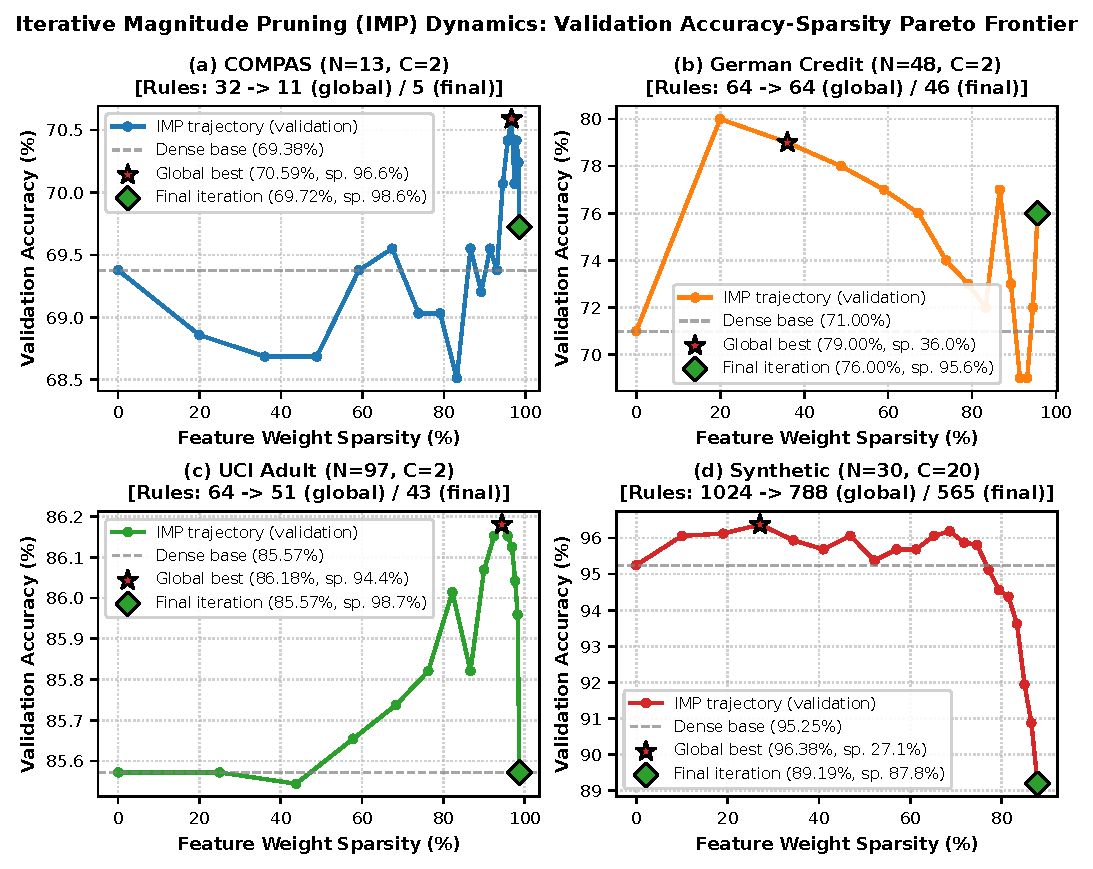
\includegraphics[width=0.95\textwidth]{figures/fig_pruning_trajectory.pdf}
\caption{Iterative magnitude pruning trajectories. Each point is one pruning
iteration; the horizontal axis is feature-connection sparsity and the vertical
axis is validation accuracy. Stars mark the validation-selected Global Best
checkpoint and diamonds the final Compact checkpoint. Pruning removes a large
fraction of connections while the validation accuracy remains in a narrow band;
the final iterations of German Credit and Synthetic show the expected increase in
variance as the rule set becomes very small.}
\label{fig:pruning_trajectory}
\end{figure*}

\subsubsection{Rule Counts and Rule Length}
The effect of pruning is dataset-dependent. On COMPAS, 32 initial rules collapse
to 11 (Global Best) or 5 (Compact), with 1.27 and 1.20 features per rule and
96.6\% and 98.6\% connection sparsity; the Compact model has 28 active
parameters. On German Credit the Compact model retains 46 of 64 rules with 2.70
features per rule and 96.0\% sparsity (310 active parameters), whereas the Global
Best checkpoint keeps all 64 rules with 30.72 features per rule; validation
accuracy on this dataset peaks in the first pruning iterations, so the accuracy
ceiling is a dense model. This is why we separate the two checkpoints instead of
reporting a single ``pruned'' model. On UCI Adult, 64 rules reduce to 51 and 43,
with 6.86 and 1.91 features per rule and 94.4\% and 98.7\% sparsity. On
Synthetic, 1{,}024 initial rules reduce to 788 and 565, with 26.29 and 6.61
features per rule; the 20-class problem requires substantially longer rules,
which is why the synthetic scorecard has a wider
integer range (Section~\ref{subsec:quantization_fidelity}).
Across the three binary benchmarks, the Compact models use between 5 and 46 rules
and between 1.20 and 2.70 features per rule, which is the scenario in which
rule-by-rule auditing is realistic. The parameter counts above are active
parameters: weight entries with magnitude above $10^{-4}$, plus all rule
centers, widths and output biases. They are not the dense $H\times N$ storage
footprint. The current implementation keeps the surviving rules as dense
$H\times N$ matrices, so storage and dense-kernel arithmetic scale with
$H\times N$; connection sparsity is an auditability property, not a speedup that
the kernel realizes. The synthetic model is deliberately kept as a capacity
benchmark and is not presented as a human-auditable artifact.

\subsubsection{Dual-Device Latency}
Because the compact model retains only a few rules and features per rule, its
forward pass is small and inference is inexpensive
(Table~\ref{tab:computational_efficiency}). On the host CPU a \emph{single
query} (batch $=1$) takes 59.4--84.4~$\mu$s, while batch inference over an entire
test set for the Compact model takes 0.08--6.72~ms, the upper end being the
Synthetic test set (4{,}000 samples). At these sizes the single-query gap is
per-call framework overhead, not arithmetic. On the GPU, kernel-launch overhead
dominates (347--384~$\mu$s; the input tensor is preloaded, so host-to-device
transfer is excluded), so the CPU is faster for online scoring and the GPU pays
off only for large batches, where it is about $6.7\times$ faster on Synthetic.

On the amortized per-instance metric (batch latency divided by the number of test
examples) \modelname{} processes one German Credit instance in 0.8~$\mu$s,
against 1.1--364.8~$\mu$s for the 13 baselines measured under the same host CPU
and test set (Supplementary Table~S4). The representative gradient-boosted
ensembles are 4--10 times slower, whereas Random Forest and AdaBoost are about
300 and 440 times slower. Each model is timed through its own prediction API, so
the comparison reflects library-default threading and call overhead rather than a
thread-matched kernel benchmark. A single query is less favorable: per-call
overhead dominates and \modelname{} needs about 60~$\mu$s
(Table~\ref{tab:computational_efficiency}). Single-query baselines were not
measured, so the two definitions are not interchangeable. The SCORE-Net batch
standard deviation is below 0.03~$\mu$s per sample, so the gap to logistic
regression (1.4~$\mu$s) is well above measurement noise. Random Forest is at most
1.0 point more accurate here but more than two orders of magnitude slower per
instance.

Training cost is a different matter. A full pruning trajectory takes about
0.23~min on German Credit, 2.9~min on COMPAS, 5.2~min on UCI Adult and 7.9~min on
Synthetic, averaged over the cross-validation folds (Supplementary Table~S3).
The trajectory contains the base fit plus 14--20 pruning stages, so the per-stage
cost is comparable to a single baseline fit; on Synthetic the two are almost
equal, while the baselines are cheaper on the other three datasets. The compact
structure is therefore paid for once, offline, and is not free at training time.

\subsection{Integer Scorecard Fidelity}
\label{subsec:quantization_fidelity}

\begin{table*}[!tb]
\centering
\footnotesize
\caption{Float versus rule-level integer scorecard. Only $W_f$ is quantized; $W_o$ stays continuous. Fidelity is instance-level prediction agreement and $\Delta\text{Acc}$ is the difference of the two displayed accuracies. The last block is the no-protected COMPAS variant.}
\label{tab:scorecard_fidelity}
\renewcommand{\arraystretch}{1.3}
\setlength{\tabcolsep}{3pt}
\adjustbox{max width=\linewidth}{%
\begin{tabular}{llccccccc}
\toprule
\textbf{Dataset} & \textbf{Variant} & \textbf{Rules ($H^*$)} & \textbf{Float Acc (\%)} & \textbf{Scorecard Acc (\%)} & \textbf{$\Delta$ Acc (\%)} & \textbf{Fidelity (\%)} & \textbf{Weight Range} & \textbf{Mean $\bar{\lambda}$} \\
\midrule
\multirow{2}{*}{COMPAS} & Global Best & 11 & 68.33 & 68.40 & +0.07 & 99.79 & $[-3, 3]$ & 6.27 \\
 & Compact & 5 & 66.32 & 66.32 & 0.00 & 100.00 & $[-3, 3]$ & 7.60 \\
\midrule
\multirow{2}{*}{German Credit} & Global Best & 64 & 76.00 & 77.00 & +1.00 & 97.00 & $[-9, 8]$ & 29.11 \\
 & Compact & 46 & 75.00 & 76.00 & +1.00 & 97.00 & $[-5, 6]$ & 15.00 \\
\midrule
\multirow{2}{*}{UCI Adult} & Global Best & 51 & 85.30 & 85.36 & +0.06 & 98.76 & $[-8, 7]$ & 35.29 \\
 & Compact & 43 & 85.61 & 85.54 & -0.07 & 99.40 & $[-7, 4]$ & 25.02 \\
\midrule
\multirow{2}{*}{Synthetic} & Global Best & 788 & 95.78 & 94.68 & -1.10 & 96.63 & $[-21, 22]$ & 138.97 \\
 & Compact & 565 & 90.03 & 89.23 & -0.80 & 95.45 & $[-20, 24]$ & 106.88 \\
\midrule
\multirow{2}{*}{COMPAS (no sex/race)} & Global Best & 25 & 68.68 & 68.61 & -0.07 & 99.24 & $[-7, 7]$ & 16.80 \\
 & Compact & 3 & 66.67 & 66.60 & -0.07 & 99.51 & $[-1, 3]$ & 5.00 \\
\bottomrule
\end{tabular}
}
\end{table*}


\subsubsection{Adaptive Scaling versus Global Scaling}
A small global multiplier destroys accuracy: with $\lambda \le 2$ many weights
round to zero and accuracy falls to 70.00\%. Accuracy returns to the float level
for $\lambda \ge 10$, with a visible dip at $\lambda = 100$ caused by rounding a
few borderline cases, but a large uniform multiplier inflates the integer range:
at $\lambda = 1000$ the point span approaches 700, which makes manual scoring
impractical (Supplementary Figure~S2). The rule-adaptive scheme of
Equation~\eqref{eq:adaptive_scale} instead selects the smallest multiplier per
rule that satisfies a relative rounding tolerance ($\tau_{tol} = 1\%$ for German
Credit Compact). For the 46 rules this yields multipliers between 4 and 20 (mean
15.00) and integer weights confined to $[-5, 6]$.

\subsubsection{Fidelity and Agreement}
Table~\ref{tab:scorecard_fidelity} reports, for both checkpoints and all four
datasets, the float and scorecard accuracies, the accuracy change
$\Delta\text{Acc} = \text{Acc}^{(\text{quant})} - \text{Acc}^{(\text{float})}$,
the instance-level prediction agreement (Equation~\ref{eq:fidelity}), the integer
weight range and the mean multiplier. The final block repeats the measurement for
the protected-attribute-free COMPAS variant of
Section~\ref{subsec:comparative_results}, whose three Compact rules appear in
Figures~\ref{fig:arch_forward}--\ref{fig:arch_scorecard} and in the case study.
Four observations follow.
\begin{enumerate}
    \item \textbf{Agreement is high but not exact.} Fidelity ranges from 95.45\%
    (Synthetic Compact) to 100.00\% (COMPAS Compact). This is an empirical
    property of rounding, not a theorem; unlike the bias-shifting step, integer
    quantization does not preserve logits exactly.
    \item \textbf{Accuracy changes are small and not systematic.} On COMPAS and
    Adult the absolute change is at most 0.07 points; on German Credit the
    scorecard is 1.00 point \emph{more} accurate than the float model, which is
    within one example of noise on a 100-example test set; on Synthetic the
    scorecard loses 0.80--1.10 points. We report the sign as measured.
    \item \textbf{The integer range tracks the number of classes and rule
    length.} Binary problems with short rules need only a handful of points
    ($[-3,3]$ on COMPAS, $[-5,6]$ on German Credit Compact, $[-7,4]$ on Adult
    Compact), whereas the 20-class problem with rules of length 6.6 requires
    $[-20,24]$.
    \item \textbf{Removing the protected attributes does not change the picture.}
    With budgets chosen by the same fidelity/span criterion (10/3\% for Compact,
    30/5\% for Global Best), the variant reaches 99.51\% (3-rule Compact) and
    99.24\% (25-rule Global Best) agreement, with a $-0.07$-point accuracy change
    in both cases.
\end{enumerate}
On every binary benchmark, including the no-protected COMPAS variant, the pruned
model therefore admits a small-integer scorecard with at least 97\% prediction
agreement and an accuracy change of at most one percentage point, while the output
layer remains continuous and interpretable as signed votes.

\subsection{Transparent Case Studies and Decision Diagnostics}
\label{subsec:case_studies}

\subsubsection{Pencil-and-Paper Scorecard: COMPAS}
Figure~\ref{fig:compas_pencil_paper_scorecard}(a) lists the complete Compact model
for the protected-attribute-free COMPAS variant: three univariate interval rules
on \textit{priors\_count} ($\le 4.3$), \textit{juv\_misd\_count} ($\le 0.4$) and
\textit{age} ($\le 25.6$). No rule conditions on race or sex. The output layer
contributes signed votes per class plus a base bias ($-0.23$ for non-recidivism,
$+0.17$ for recidivism) created by the bias-shifting step.

Panel (b) audits two defendants by hand. Defendant~A (\textit{priors} = 0,
\textit{juv\_misd\_count} = 0, \textit{age} = 40) activates $R_1$ and $R_2$ but not
the age rule $R_3$, and the rule votes plus the bias give $+0.43$ for
non-recidivism and $-0.64$ for recidivism, a margin of 1.07. Defendant~B
(\textit{priors} = 5, \textit{juv\_misd\_count} = 3, \textit{age} = 19) activates
only $R_3$, giving $-1.01$ and $+0.93$, a margin of 1.94 for recidivism. Both
decisions match the network output exactly, because the decomposition is an
algebraic identity rather than a surrogate. Panel (c) places the three-rule and
25-rule models next to the baselines on the accuracy axis.

\begin{figure*}[t]
\centering
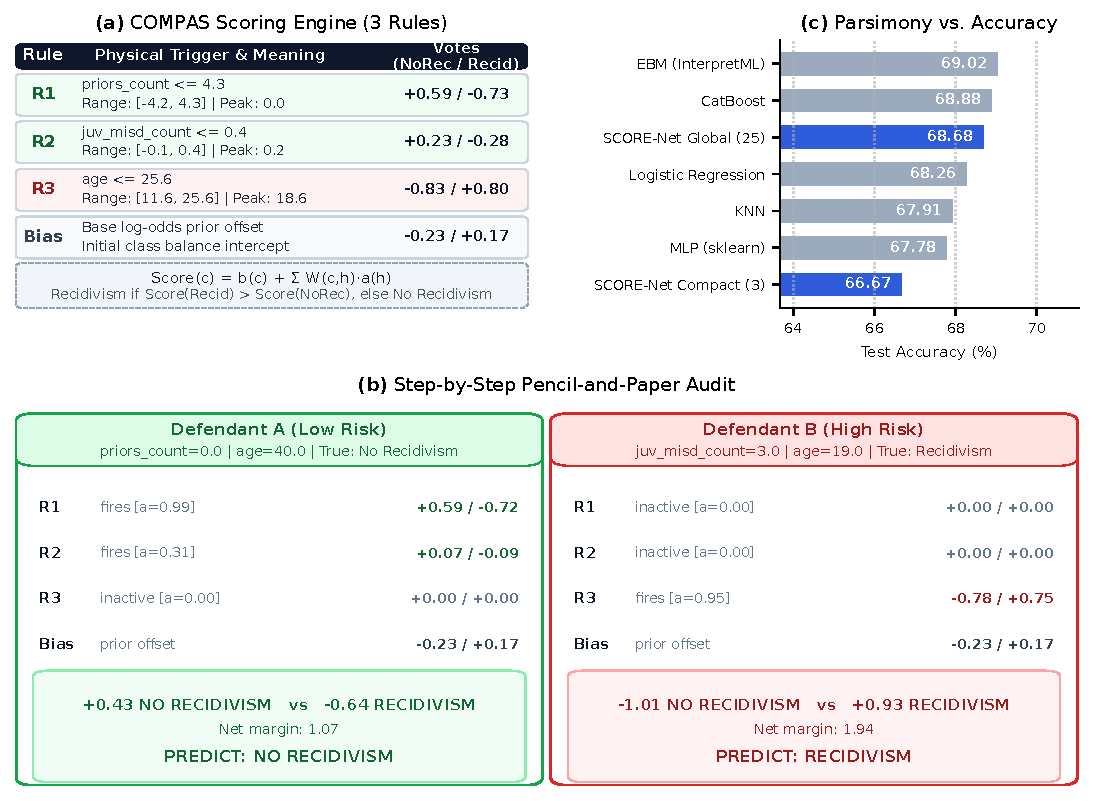
\includegraphics[width=0.94\textwidth]{figures/fig_compas_pencil_paper_scorecard.pdf}
\caption{Pencil-and-paper audit of the three-rule \modelname{} model on the
protected-attribute-free COMPAS variant. (a) Rules, activation intervals and signed
output votes; none of the rules conditions on race or sex.
(b) Step-by-step arithmetic for a low-risk and a high-risk defendant; the
reconstructed scores equal the network logits exactly. (c) Accuracy of the
three-rule and 25-rule models relative to the baselines.}
\label{fig:compas_pencil_paper_scorecard}
\end{figure*}

\subsubsection{Decision Diagnostics: German Credit}
The same diagnostic tools apply to the German Credit model. For a rejected
applicant with decision margin $-0.54$, the exact response curve of
\textit{duration} crosses the boundary at $-0.17$ standard deviations, so a shift
of $-0.42$ suffices for approval, while \textit{credit\_amount} is non-monotone
and opens an approval corridor on roughly $[0.69, 1.87]$. The closed-form
recourse search then returns independent single-feature interventions, the
smallest being a reduction of \textit{residence\_since} by 0.35 and of
\textit{duration} by 0.42 standard deviations; because each root solves a
piecewise-linear equation, the shifts are exact for the model. Finally,
off-diagonal Jaccard similarities between the ten most used features are at most
0.33, consistent with the average rule length of 2.70 features: pruning decouples
most features into short, individually auditable rules. These remain
\emph{geometric} diagnostics, not causal claims. The three figures are given in
Supplementary Section~S7 (Figures~S3--S5).

\subsection{Stability of the Extracted Rules}
\label{subsec:stability}

A rule set that changes completely between runs is not auditable, so we retrain
COMPAS and German Credit with five seeds, holding the split and every
hyperparameter fixed, and compare the rule sets pairwise. Both checkpoints are
measured. \emph{Global Best} is the validation-selected iteration, so its depth
follows each seed's validation curve and can stop before pruning bites;
\emph{Compact} always runs the full schedule, so all seeds are compared at the
same sparsity. Table~\ref{tab:seed_stability} gives, for each, the overlap over
rule \emph{signatures} and over the features used by at least one rule.

The two overlaps diverge, and the divergence is the finding. For the
validation-selected checkpoint the feature support is almost perfectly stable: on
COMPAS every seed selects the same 13 features (Jaccard $1.00$) and on German
Credit the overlap is $0.91 \pm 0.04$, while rule signatures barely repeat
($0.13 \pm 0.12$ and $0.02 \pm 0.01$). Its rule count reflects the selected depth
rather than a budget: COMPAS keeps $31.8 \pm 0.4$ of the $32$ initial units
because validation peaks before pruning removes whole units, and German Credit
keeps $52.4 \pm 4.0$ of $64$.

The compact operating point separates what Global Best conflates. Its connection
budget is fixed by the schedule (six weights on COMPAS, five or six observed
across the five seeds; $134$--$135$ on German Credit), so the seed changes the
grouping of the budget rather than its size. On COMPAS that budget becomes
$5.0 \pm 0.7$ rules over three to five features, matching the five-rule Compact
model of Section~\ref{subsec:comparative_results}. Rule-set overlap rises to
$0.38 \pm 0.15$ and feature overlap falls to $0.40 \pm 0.18$: every run spends
the same small budget on a small coherent subset, but \emph{which} subset is
seed-dependent. On German Credit, where pruning is milder, Compact keeps
$50.6 \pm 2.9$ of $64$ rules with overlaps close to Global Best
($0.04 \pm 0.02$, $0.88 \pm 0.04$).

This is the clearest limitation of the present work and we do not soften it. A
rule reported for one run is one member of a family of equally accurate rules,
not a uniquely determined explanation. The per-example decomposition of
Section~\ref{subsec:analytical_xai} is unaffected, because it is an identity for
whichever model is loaded; what is not guaranteed is that retraining reproduces
the same rule list. Stability-aware pruning objectives are the natural next step.

\begin{table*}[t]
\centering
\footnotesize
\caption{Rule-set stability over five seeds (means over the 10 seed pairs). \emph{Global Best} is the validation-selected iteration; \emph{Compact} runs the full schedule. \emph{Rule set} and \emph{Features} are Jaccard overlaps over rule signatures and over the features used by at least one rule; \emph{Links} is the surviving weight count.}
\label{tab:seed_stability}
\setlength{\tabcolsep}{6pt}
\renewcommand{\arraystretch}{1.05}
\adjustbox{max width=\linewidth}{%
\begin{tabular}{l l c c c c c}
\toprule
\textbf{Dataset} & \textbf{Checkpoint} & \textbf{Rules ($H^*$/$H_0$)} & \textbf{Links} & \textbf{Rule set} & \textbf{Features} & \textbf{Acc (\%)} \\
\midrule
\multirow{2}{*}{COMPAS} & Global Best & 31.8$\pm$0.4 / 32 & 266--414 & 0.13$\pm$0.12 & 1.00$\pm$0.00 & 67.14$\pm$0.41 \\
 & Compact & 5.0$\pm$0.7 / 32 & 5--6 & 0.38$\pm$0.15 & 0.40$\pm$0.18 & 66.03$\pm$0.56 \\
\multirow{2}{*}{German Credit} & Global Best & 52.4$\pm$4.0 / 64 & 134--210 & 0.02$\pm$0.01 & 0.91$\pm$0.04 & 72.00$\pm$2.00 \\
 & Compact & 50.6$\pm$2.9 / 64 & 134--135 & 0.04$\pm$0.02 & 0.88$\pm$0.04 & 72.80$\pm$3.03 \\
\bottomrule
\end{tabular}
}
\end{table*}



\subsection{Ablation Studies and Sensitivity Analysis}
\label{subsec:ablations}

\subsubsection{Loss Regularization and Dropout}
Table~\ref{tab:ablation_synthetic} and Supplementary Figure~S6a
isolate the contribution of the two $\ell_1$ penalties and of dropout on the
Synthetic benchmark with $H_{\text{init}} = 1024$. The full model reaches 90.03\%
with 565 surviving rules (44.8\% pruned).
\begin{itemize}
    \item Removing the feature penalty ($\lambda_1 = 0$) drops accuracy to
    70.13\% ($-19.90$) with 999 rules essentially unpruned: without input
    sparsity pruning cannot shorten rules, and both compactness and accuracy go.
    \item Removing the output penalty ($\lambda_2 = 0$) gives 66.72\%
    ($-23.31$) with 970 rules, so rule-level sparsity is not a by-product of
    input pruning alone.
    \item Removing both penalties collapses accuracy to 57.78\% ($-32.25$) with
    1{,}003 rules.
    \item Removing dropout slightly \emph{raises} accuracy (91.22\%, $+1.19$) and
    prunes more aggressively (437 rules survive) but lengthens the average rule from 6.6 to 8.5
    features; dropout is kept for rule brevity, not accuracy.
\end{itemize}

\begin{table*}[t]
\centering
\footnotesize
\caption{Ablation study on the multi-class Synthetic benchmark (20 classes, 30 features). We vary individual loss regularization components and the initial model capacity $H$ and report test accuracy, rule pruning, feature sparsity and average rule length.}
\label{tab:ablation_synthetic}
\setlength{\tabcolsep}{3pt}
\adjustbox{max width=\linewidth}{%
\begin{tabular}{l ccc ccc c}
\toprule
\textbf{Ablation Variant} & \textbf{Initial $H$} & \textbf{Pruned $H^*$} & \textbf{Pruning (\%)} & \textbf{Feat. Sparsity (\%)} & \textbf{Avg. Feat/Rule} & \textbf{Test Acc. (\%)} & \textbf{$\Delta$ Acc. (\%)} \\
\midrule
\multicolumn{8}{l}{\textit{\textbf{Loss Regularization and Dropout Ablation ($H_{\text{init}}=1024$)}}} \\
SCORE-Net (Full Dual $L_1$, H=1024) & 1024 & 565 & 44.8\% & 78.0\% & 6.6 & \textbf{90.03\%} & \textit{Baseline} \\
No Dropout ($p = 0.0$) & 1024 & 437 & 57.3\% & 71.5\% & 8.5 & 91.22\% & +1.19\% \\
No Feature $L_1$ ($\lambda_1 = 0$) & 1024 & 999 & 2.4\% & 87.8\% & 3.7 & 70.13\% & -19.90\% \\
No Output $L_1$ ($\lambda_2 = 0$) & 1024 & 970 & 5.3\% & 87.2\% & 3.9 & 66.72\% & -23.31\% \\
No $L_1$ Loss ($\lambda_1 = \lambda_2 = 0$) & 1024 & \textbf{1003} & 2.1\% & 87.6\% & 3.7 & 57.78\% & -32.25\% \\
\midrule
\multicolumn{8}{l}{\textit{\textbf{Initial Capacity Scaling ($H$)}}} \\
Low Capacity ($H=512$) & 512 & 393 & 23.2\% & 84.2\% & 4.8 & 75.75\% & -14.28\% \\
Standard Capacity ($H=1024$) & 1024 & 565 & 44.8\% & 78.0\% & 6.6 & \textbf{90.03\%} & \textit{Baseline} \\
High Capacity ($H=2048$) & 2048 & \textbf{688} & 66.4\% & 63.9\% & 10.8 & 95.60\% & +5.57\% \\
\bottomrule
\end{tabular}
}
\end{table*}


\subsubsection{Initial Capacity}
The initial rule pool varies the same trade-off (Supplementary Figure~S6b). With
$H_{\text{init}} = 512$ the model reaches 75.75\% with 393 rules (23.2\% pruned);
with $H_{\text{init}} = 1024$ it reaches 90.03\% with 565 rules; with
$H_{\text{init}} = 2048$ it reaches 95.60\% with 688 rules (66.4\% pruned, average
length 10.8). A larger initial pool therefore improves the quality of the
surviving rules, consistent with the lottery-ticket view of
pruning~\cite{frankle2018lottery}, at the cost of longer training and longer
rules. This is a capacity--auditability trade-off, not a free improvement.

\subsubsection{Empirical Validation of the Bias-Shifting Proposition}
Table~\ref{tab:theorem1_bias_shifting} compares the exact bias-shifting
compaction of Proposition~\ref{prop:bias_shifting} with naive removal of
structurally empty rules. Only structurally empty rules are removed, so the only
difference between the two variants is the bias update. With the exact shift, the
maximum logit drift is between $8.94 \times 10^{-8}$ and $5.72 \times 10^{-6}$,
i.e., at floating-point level plus the effect of the $10^{-4}$ emptiness
threshold, and prediction agreement is 100.00\% on every dataset. Without the
shift, test accuracy falls by 9.01 points on COMPAS (66.32\% $\to$ 57.31\%) and by
2.00 points on German Credit (75.00\% $\to$ 73.00\%). On Synthetic the pruned
output weights are already negligible, so naive removal happens to be harmless.
The correction is therefore not cosmetic.

\begin{table*}[t]
\centering
\footnotesize
\caption{Exact bias shifting versus naive removal of structurally empty rules, so the only difference is the bias update. Proposition~\ref{prop:bias_shifting} preserves the output up to floating-point and threshold effects (maximum drift $5.72 \times 10^{-6}$).}
\label{tab:theorem1_bias_shifting}
\setlength{\tabcolsep}{6pt}
\adjustbox{max width=\linewidth}{%
\begin{tabular}{l c cc cc c}
\toprule
\multirow{2}{*}{\textbf{Dataset}} & \multirow{2}{*}{\textbf{Pruned Rules}} & \multicolumn{2}{c}{\textbf{Proposition~\ref{prop:bias_shifting} (Exact Shift)}} & \multicolumn{2}{c}{\textbf{Naive Pruning (No Shift)}} & \multirow{2}{*}{\textbf{Drift Penalty}} \\
\cmidrule(lr){3-4} \cmidrule(lr){5-6}
 & & \textbf{Max Drift} & \textbf{Fidelity} & \textbf{Max Drift} & \textbf{Fidelity} & \\
\midrule
COMPAS & 27 / 32 & $1.19 \times 10^{-7}$ & 100.00\% & 0.3647 & 62.44\% & +9.01\% \\
COMPAS (no protected attributes) & 29 / 32 & $8.94 \times 10^{-8}$ & 100.00\% & 0.2274 & 63.55\% & +8.59\% \\
German Credit & 12 / 64 & $4.77 \times 10^{-7}$ & 100.00\% & 0.2482 & 92.00\% & +2.00\% \\
UCI Adult & 21 / 64 & $7.15 \times 10^{-7}$ & 100.00\% & 0.1543 & 96.98\% & +0.48\% \\
Synthetic & 459 / 1024 & $5.72 \times 10^{-6}$ & 100.00\% & 0.0001 & 100.00\% & +0.00\% \\
\bottomrule
\end{tabular}
}%
\end{table*}


\subsection{Limitations and Threats to Validity}
\label{subsec:limitations}

Several limitations bound the claims of this paper.
\begin{itemize}
    \item \textbf{Not uniformly more accurate.} On the single split \modelname{}
    is statistically indistinguishable from the strongest baseline on COMPAS
    (Global Best) and German Credit, but the shared folds place it 2.8--3.1 points
    behind CatBoost on German Credit and 1.52--1.85 behind the best
    gradient-boosted ensemble on UCI Adult ($p < 0.001$). The synthetic result
    reflects a generator whose geometry matches convex slabs and should not be
    generalized to arbitrary tabular data.
    \item \textbf{Small test sets.} German Credit has 100 test examples, so one
    example is one percentage point. Bootstrap intervals, McNemar tests and a
    $5\times5$ cross-validation mitigate this, and the cross-validated mean is
    reported alongside the single split.
    \item \textbf{Single seed and split sensitivity.} The single-split numbers come
    from one seeded run per dataset. On COMPAS and Adult the folds give a gap
    within half a point of the single-split gap, but on German Credit the single
    split shows parity while the folds do not, because the German budgets were
    chosen on this 1{,}000-example dataset; we therefore treat the cross-validated
    number as the expected German performance. Seed-level rule stability is the
    most important remaining limitation (Section~\ref{subsec:stability}).
    \item \textbf{Oblique rules are not automatically simple.} A rule with three or
    more active features takes more effort to check than a univariate threshold,
    even when the rule count is small; the German Global Best model, with 30.72
    features per rule, shows that a low rule count alone is not sufficient for
    auditability.
    \item \textbf{Timing is not a controlled hardware benchmark.} Latencies come
    from one 6-core laptop CPU and one entry-level GPU, with library-default
    threading. They support order-of-magnitude statements, not portable speed
    ratios. The baseline comparison covers only German Credit, whose 100-example
    test set makes per-call overhead a large fraction of the batch time. Because
    the compact model is stored densely, its measured latency reflects
    $H\times N$ arithmetic; connection sparsity is an auditability property, not a
    speedup that the current kernel exploits.
    \item \textbf{Two operating points are test-informed.} The German Credit
    pruning depth (14 instead of 20 iterations) and the quantization budget
    $(\Lambda_{\max}, \tau_{tol})$ were fixed with the single split available, so
    the single-split figures are operating points and the reported fidelity is not
    a held-out estimate. Repeating the German Credit $5\times5$ cross-validation
    at 20 iterations gives $72.90\pm2.47\%$ (Global Best) and $72.94\pm2.18\%$
    (Compact), so the depth choice moves the cross-validated mean by at most 0.2
    points. The bias-shifting step itself is exact; integer rounding is not.
    \item \textbf{Recourse is geometric.} The closed-form roots give the nearest
    model-boundary crossing under fixed remaining features and immutable
    attributes; they encode no causal dependencies, costs or feasibility.
    \item \textbf{No fairness claim.} COMPAS demonstrates transparency on a
    high-stakes dataset. We do not evaluate group fairness, and a transparent model
    is not automatically a fair one.
\end{itemize}


% --- Section 5: Conclusion ---
\section{Conclusion}
\label{sec:conclusion}

In this paper we introduced \modelname{}, an inherently interpretable neural
network for tabular classification. High-stakes applications in medicine, finance
and criminal justice require models that are both reasonably accurate and
auditable, and \modelname{} addresses this trade-off geometrically: instead of
unbounded activations such as ReLU, each hidden unit applies a localized
triangular response to a bias-free linear projection. The unit is therefore active
only inside a convex slab bounded by two parallel hyperplanes, and it can be read
as an oblique interval rule with a signed vote per class.

To keep the rule set compact, we combine dual $\ell_1$ regularization with
iterative magnitude pruning. Pruning is a structural mechanism rather than only
compression: zeroing input connections removes features from a rule, and zeroing
an entire row removes the rule. We proved the \emph{exact bias-shifting property
for pruned rules} (Proposition~\ref{prop:bias_shifting}), so a structurally empty
rule can be absorbed into the output bias with zero logit drift; without the
correction, naive removal costs up to 9.01 accuracy points. Rule-adaptive integer
quantization then converts projection weights into small integers, so compact rule
sets can be scored by hand while the output layer remains continuous and
interpretable as signed votes.

The empirical results support a bounded claim. On the single split, the COMPAS
(Global Best) and German Credit models are statistically indistinguishable from
the strongest of 13 baselines. Under the shared folds the German Credit gap is
2.8--3.1 points, and on UCI Adult the models trail the best gradient-boosted
ensemble by 1.52--1.85 points. The interpretable operating point uses 5 rules on
COMPAS, 46 on German Credit and 43 on Adult, with 1.2--2.7 features per rule. On
the 20-class synthetic task the localized-slab representation is much stronger
than tree ensembles, but that benchmark was generated from localized geometry and
should be read as a controlled demonstration rather than as evidence of general
superiority. Integer scorecards retain 95.45--100\% prediction agreement.

Several questions remain open. The architecture targets tabular classification, and
extending convex slabs to regression, survival analysis or unstructured data is
future work. Rules that combine three or more variables require more cognitive
effort than univariate thresholds, and a low rule count alone is not sufficient
for auditability, as the dense German Credit Global Best checkpoint illustrates.
Rule stability is the most important open issue: across five seeds the feature
support is nearly stable (Jaccard $0.91$--$1.00$) but individual rule signatures
are not ($0.02$--$0.13$), and the compact model reduces COMPAS to about five rules
per run with mean rule-set overlap $0.38 \pm 0.15$. A reported rule is therefore
one member of a family of equally accurate rules rather than a uniquely determined
explanation, which makes stability-aware pruning the natural next step. Iterative
pruning also increases offline training time, although deployment cost remains
low. Finally, a transparent model is not automatically a fair model: we do not
evaluate group fairness on COMPAS, and human auditing of proxy attributes remains
essential. Promising directions include causal constraints for recourse,
stability-aware pruning objectives, and compiling quantized scorecards into
low-power edge firmware.


% --- Declarations (CRediT, competing interests, data, generative AI, funding) ---
%% ---------------------------------------------------------------------------
%%  Mandatory declarations for Elsevier / Neurocomputing.
%% ---------------------------------------------------------------------------

\section*{CRediT authorship contribution statement}

\textbf{Ahmet Alkan:} Conceptualization, Methodology, Software, Validation,
Formal analysis, Investigation, Data curation, Writing -- original draft,
Writing -- review and editing, Visualization.
\textbf{Gozde Yolcu Oztel:}  Supervision,
Writing -- review and editing, Project administration.

\section*{Declaration of competing interest}

The authors declare that they have no known competing financial interests or
personal relationships that could have appeared to influence the work reported
in this paper.

\section*{Data availability}

The COMPAS, German Credit, and UCI Adult datasets are publicly available from
their original providers and are cited in the text. The synthetic benchmark is
generated by the released code, which fixes the generator and its random seed,
so the data can be reproduced exactly. The code, the trained checkpoints, and
the scripts that regenerate every table and figure in this article are openly
available at
\mbox{\url{https://github.com/aalkann/SCORE-Net}} (archived at
\mbox{\url{https://doi.org/10.5281/zenodo.24217264}}).
% SUBMISSION GATE: this statement must be true when the manuscript is submitted.
% The repository is public (build.sh verifies the link and reports HTTP 200).

\section*{Funding}

This research did not receive any specific grant from funding agencies in the
public, commercial, or not-for-profit sectors.

%% Optional: uncomment and complete if acknowledgements are desired.
% \section*{Acknowledgements}
% The authors thank ...

\section*{Declaration of AI and AI-assisted technologies in the writing process}

During the preparation of this work the authors used an AI-based writing
assistant (OpenCode, with a DeepSeek large language model) in order to improve
the language, clarity, and readability of the manuscript. After using this
tool/service, the authors reviewed and edited the content as needed and take
full responsibility for the content of the publication.


% --- Bibliography ---
% Tighten the inter-entry spacing so the list ends on the last text page;
% the font size itself is unchanged.
\setlength{\bibsep}{0pt}
\renewcommand{\bibfont}{\small}
\bibliographystyle{elsarticle-num}
\bibliography{references}

\end{document}
